%(où, sous le terme, \og{}configuration\fg{} on désigne l’association de la version de ROC et
%de la REN, p. ex. les résultats de la configuration Kraken-\texttt{spaCy\_lg})
\section{Évaluation de l'impact des contaminations de ROC sur la REN} 
\label{subsec:OCR-IMPACT-NER}
\subsection{Outils de ROC et REN utilisés dans le cadre de cette étude}
\textbf{Afin de produire différentes transcriptions de ROC, nous avons utilisé deux systèmes disponibles gratuitement : Kraken \cite{kiessling2019kraken} et Tesseract \cite{smith2007overview}. Kraken est un outil pour lequel il existe différents modèles neuronaux,
dont un modèle pour le français du XVII\ieme{}siècle \cite{gabay:hal-02577236}\footnote{\url{https://github.com/Heresta/OCR17plus/tree/main/Model}} 
%ainsi qu'un modèle HTR\footnote{Abbr. angl. \textit{Handwritten Text Recognition} ou la reconnaissance d'écriture manuscrite, basée sur l'extraction du texte à partir des blocs textuels (lignes), contrairement à la méthode de ROC qui traite les caractères individuelles \cite{gabayscicos}.}
ainsi que le modèle Gallicorpora \cite{pinche_2022_7410529}. Concernant Tesseract nous avons utilisé le modèle LSTM \texttt{tessdata\_best}, entraîné sur des données Google. Tesseract propose une analyse de la mise en page intégrée à travers la segmentation des cadres (angl. \textit{box segmentation}), ce qui rend le traitement des mises en page complexes plus difficile \cite{reul2017case}.}. C'est un outil qui présente toujours de bonnes performances dans sa configuration par défaut \cite{clausner2020efficient}, qui est semble-t-il en fait un modèle entrainé pour l'anglais. Quatre modèles de langue neuronaux pour la ROC ont été utilisés dans le cadre des expériences : le modèle de base de Kraken qui permet d'opérer la segmentation\footnote{Le modèle de segmentation est constitué d'un réseau d'étiquetage en graines (angl. \textit{seed-labeling network}), qui est un \textit{U-net} (\og{}réseau entièrement convolutionnel\fg{}) modifié \cite{ronneberger2015} sur la base d'un réseau neuronal résiduel (ResNet) à 34 couches \cite{he2016}, pré-entraîné sur ImageNet.} et la transcription\footnote{Le modèle de transcription fonctionne comme un classificateur de séquences sans segmentation qui utilise un réseau neuronal artificiel pour mapper une image d'une ligne de texte (séquence d'entrée), en une séquence de caractères (séquence de sortie). Le réseau de neurones convolutif et récurrent a été entraîné avec la fonction de perte CTC (angl. \textit{Connexionist Temporal Classification} \cite{graves2006connectionist}).} d'un PDF, et
%\footnote{Le modèle par défaut de Tesseract est l'anglais. Nous précisons la langue Tess. eng, Tess. fr et Tess. suivant les bonnes pratiques de \#RègledeBender \cite{bender-friedman-2018-data}.} et (iii) 
les trois modèles Tesseract pour l'anglais, le français et le portugais contemporain\footnote{\url{https://doc.ubuntu-fr.org/tesseract-ocr}}.

\textbf{Pour effectuer la tâche de REN nous avons utilisé les chaînes de traitements de la boîte à outils pour le TAL  \texttt{spaCy}\footnote{version 3.5.1}.
% \texttt{spaCy}\footnote{version 3.5.1} et \texttt{stanza}\footnote{1.5.0}. 
Le système \texttt{spaCy} contient une stratégie d'intégration de mots utilisant des fonctionnalités de sous-mots et les plongements ``Bloom'' (angl. \textit{Bloom embeddings})\footnote{Il s'agit de la structure de données probabiliste qui permet de réduire la dimension des vecteurs (\textit{cf.} \url{https://explosion.ai/blog/bloom-embeddings}).}, ainsi qu'un réseau neuronal convolutif avec des connexions résiduelles, ce qui peut expliquer sa robustesse lors de l'extraction des EN contaminées. \texttt{spaCy} propose des modèles de langue du type \textit{large} pour le français\footnote{\url{https://spacy.io/models/fr}, \texttt{fr\_core\_news\_lg}}, le portugais\footnote{\url{https://spacy.io/models/pt}, \texttt{pt\_core\_news\_lg}} et l'anglais\footnote{\url{https://spacy.io/models/en}, \texttt{en\_core\_web\_lg}}. Nous avons favorisé l'usage du modèle \textit{large} (\texttt{spaCy\_lg}) plutôt que du modèle \textit{small} (\texttt{spaCy\_sm}) car la différence principale entre les deux modèles pour les trois langues tient à l'ajout de la vectorisation et des plongements de mots (angl. \textit{embeddings}) dans l'entraînement du modèle \textit{large}\footnote{Modèle anglais : Explosion Vectors (OSCAR 2109 + Wikipedia + OpenSubtitles + WMT News Crawl) (Explosion). Modèles français et portugais :
Explosion fastText Vectors (CBOW, OSCAR Common Crawl + Wikipedia) (Explosion).}}.


\subsection{Typologie des contaminations et problèmes d'alignement}



Dans un premier temps, nous proposons une évaluation de l'outil de REN \texttt{spaCy} sur données bruitées, dans laquelle nous comparons les résultats obtenus sur les sous-corpus ELTeC français, anglais et portugais et la TGB, et, leurs transcriptions de ROC\footnote{Dépôt github avec nos données : \url{anonymous}} sans nous appuyer sur un \textit{gold standard}.

Nous observons que les fautes d'orthographes provoquées par la ROC ne sont pas systématiquement un frein à la bonne extraction des noms de lieux, comme en témoigne le tableau \ref{tab:typo_erreurs_ocr}. En revanche, la concaténation des tokens d'une EN semble être une contamination plus préjudiciable à sa bonne détection. Par ailleurs, l'étude de \cite{DBLP:conf/gis/Koudoro-Parfait21} laisse entendre que (i) le contexte contaminé autour d'une EN pourrait être un facteur de non détection et (ii) un contexte parfaitement propre ne serait pas la garantie que l'EN soit reconnue par le système. Il semble que ces faits soient vérifiables pour les trois langues sur lesquelles nos expériences ont porté. Par ailleurs, certaines entités même très contaminées sont identifiées, comme p.\ ex.\  \textit{``ancehester''} (pour \og{}Manchester\fg{}). 

\begin{table}[h!]
\small
    \centering
   %%%%%%%%%%% Ancien tableau avec stanza, 07/02/2024 %%%%%%%%%%%%%%%
%
%\scriptsize{\begin{tabular}{|p{3.2cm}|p{4cm}|p{1.5cm}|p{1.3cm}|}
%
%%\multicolumn{5}{|c|}{Results for Named Entities Recognition} \\
%\hline
%
%
%\bf{Impact types} & \bf {contexte} &  \bf{\texttt{spaCy\_lg}}&\bf{\texttt{stanza}}\\
%\hline
% Contamination orthographique interne à l'entité& 
%\textit{il en est tombe au sort cinq de Sain\textcolor{red}{l}-Brun\textcolor{red}{c}lle} & Sain\textcolor{red}{l}-Brun\textcolor{red}{c}lle. & Sain\textcolor{red}{l}-Brun\textcolor{red}{c}lle \\
%
%&\textit{durant\textcolor{red}{a} todo o t\textcolor{red}{o}mpe
%em q\textcolor{red}{n}e ostivess\textcolor{red}{o} em Port\textcolor{red}{n}gal}& Port\textcolor{red}{n}gal & N/A\\ 
%&&  & \\
%\rowcolor{lightgray}ajout d'un caractère minuscule au début de l'entité &\textit{Aux \textcolor{red}{k}Etats-Unis}& \textcolor{red}{()} & \textcolor{red}{k}Etats-Unis\\
%&&  & \\
%ponctuation substituée par un caractère collé à l'entité &\textit{about Manchester\textcolor{red}{l} A
%pretty state}&Manchester\textcolor{red}{l}&Manchester\textcolor{red}{l}\\
%&&  & \\
%\rowcolor{lightgray}Entité tronquée &\textit{dans l'intérieur de l'Améri-} & Améri—& \textcolor{red}{()}\\
%\rowcolor{lightgray}&\textit{et le golfe de Cali-foruie.\_n}&golfe de Cali-& golfe de Cali-\\
%&&  & \\
%mots concaténés & \textit{[...] \textcolor{red}{larue} Saint-Honoré;}& \textbf{\_} Saint-Honoré &  \textcolor{red}{()} \\
%&\textit{afriver \textcolor{red}{a}Morlincourt' tot}& \textcolor{red}{()} & \textcolor{red}{()}\\
%
%
%
%% &- point d'exclamation remplacé par une lettre &\textit{Louis Quatorze might have bestowed on the ambassador
%% of the United Provinces}& N/A &theUnitedProvinces\\
%\hline
%\end{tabular}}
%%%%%%%%%%%%% Nouveau tableau sans stanza, 07/02/2024 %%%%%%%%%%%%%

\scriptsize{\begin{tabular}{|p{3.2cm}|p{4cm}|p{1.5cm}|}

%\multicolumn{5}{|c|}{Results for Named Entities Recognition} \\
\hline


\bf{Impact types} & \bf {contexte} &  \bf{\texttt{spaCy\_lg}}\\
\hline
 Contamination orthographique interne à l'entité& 
\textit{il en est tombe au sort cinq de Sain\textcolor{red}{l}-Brun\textcolor{red}{c}lle} & Sain\textcolor{red}{l}-Brun\textcolor{red}{c}lle. \\
&\textit{durant\textcolor{red}{a} todo o t\textcolor{red}{o}mpe
em q\textcolor{red}{n}e ostivess\textcolor{red}{o} em Port\textcolor{red}{n}gal}& Port\textcolor{red}{n}gal\\ 
& & \\
\rowcolor{lightgray}ajout d'un caractère minuscule au début de l'entité &\textit{Aux \textcolor{red}{k}Etats-Unis}& \textcolor{red}{()}\\
& & \\
ponctuation substituée par un caractère collé à l'entité &\textit{about Manchester\textcolor{red}{l} A
pretty state}&Manchester\textcolor{red}{l}\\
& & \\
\rowcolor{lightgray}Entité tronquée &\textit{dans l'intérieur de l'Améri-} & Améri—\\
\rowcolor{lightgray}&\textit{et le golfe de Cali-foruie.\_n}&golfe de Cali-\\
& & \\
mots concaténés & \textit{[...] \textcolor{red}{larue} Saint-Honoré;}& \textbf{\_} Saint-Honoré \\
&\textit{afriver \textcolor{red}{a}Morlincourt' tot}& \textcolor{red}{()}\\



% &- point d'exclamation remplacé par une lettre &\textit{Louis Quatorze might have bestowed on the ambassador
% of the United Provinces}& N/A &theUnitedProvinces\\
\hline
\end{tabular}}



    \caption{Proposition de typologie pour l'évaluation de la REN sur des données issues de la ROC.}
    \label{tab:typo_erreurs_ocr}
\end{table}

%%%________ Plus d'EN sur texte bruité

Le tableau \ref{tab:ELTeC_bon_mauvais} qui répertorie le nombre des types des EN reconnues par \texttt{spaCy} selon la qualité des versions de ROC, illustre le fait que sur les versions de ROC les systèmes de REN récupèrent plus de type d'EN différents, donc que la qualité du texte en entrée influe sur la quantité du type d'EN récupérées en sortie. La qualité des versions ROC a été évaluée en appliquant les métriques \textit{Character Error Rate} (CER) et \textit{Word Error Rate} (WER) sur les textes de référence et les versions de ROC. On note que plus le WER est élevé, donc plus la qualité de la transcription baisse, plus le nombre de type d'EN en sortie est élevé. On peut en conclure que le nombre des hapax augmente selon que la qualité de la transcription diminue. 
Dans la quantité d'EN surnuméraire détectée sur les versions de ROC par rapport à la référence, figurent des Faux Positifs (FP) (du bruit) mais aussi des formes contaminées des entités, qui sont des hapax, et qui comptent chacune pour un type différent d'EN en plus du type initial de l'EN. Ces phénomènes sont illustrés dans le tableau \ref{tab:FP_VP} qui recense une annotation manuelle des Vrais Positifs (VP) et des FP par type d'EN récupérées par \texttt{spaCy\_lg} sur l'ensemble des EN de référence et celui des versions pour Kraken et Tesseract français. On retrouve bien (i) plus de FP et (ii) plus de VP qui sont des hapax sur les transcriptions OCR que sur la référence. Il y a donc plus de types différents d'entités sur la sortie de la ROC que sur la sortie de la Réf., car, comme l'illustre le tableau \ref{tab:EN_contamines_Variantes}, les variantes d'une entités peuvent être nombreuses. 

%%%______________ Plus d'EN mais est-ce que c'est du bruit ?
\begin{table}[h!]
    \centering
    \small
    %%_________ TABLEAU PAS EN ORDRE
\resizebox{\textwidth}{!}{
\begin{tabular}{|l|ccc|ccc|ccc|}
\hline
 &
  \multicolumn{3}{c|}{Anglais} &
  \multicolumn{3}{c|}{Français} &
  \multicolumn{3}{c|}{Portugais} \\ \cline{2-10} 
%\multirow{}{}{} &
 
&
  
  \cellcolor[HTML]{FFFFFF}Reynolds &
  \multicolumn{1}{c|}{Troll.} &
  \multicolumn{1}{c|}{Brontë} &  
  \multicolumn{1}{c|}{Daudet} &
  Adam &
  \multicolumn{1}{c|}{Maup.} &
  \multicolumn{1}{c|}{Diniz} &
 Queiroz&
  \multicolumn{1}{c|}{Osorio}
   \\ \hline
\hline
% TODO les CER et WER pour kraken ne correspondent plus à la réalité des réusltats ils n'ont pas été déplacé comme ceux de tesseract


% CER Kraken\ \ &
%     \multicolumn{1}{r|}{ 0.98}&
%   \multicolumn{1}{r|}{0.47} &
%   \multicolumn{1}{r|}{0.22} &
%   \multicolumn{1}{r|}{0.05} &
%   \multicolumn{1}{r|}{0.11} &
%   \multicolumn{1}{r|}{0.15} &
%   \multicolumn{1}{r|}{0.22} &
%   \multicolumn{1}{r|}{0.10}&
%   \multicolumn{1}{r|}{0.15} 
%    \\ %\hline

%   WER Kraken\ \ &
%   \multicolumn{1}{r|}{0.99 }&
%   \multicolumn{1}{r|}{0.54} &
%   \multicolumn{1}{r|}{0.32} &
%   \multicolumn{1}{r|}{0.18} &
%   \multicolumn{1}{r|}{0.34} &
%   \multicolumn{1}{r|}{0.33} &
%   \multicolumn{1}{r|}{0.51} &
%   \multicolumn{1}{r|}{0.33}&
%   \multicolumn{1}{r|}{0.41} 
%    \\ %\hline
%    \hline

CER Tess+ lang.\ \ &
 \multicolumn{1}{r|}{0.10}&
  \multicolumn{1}{r|}{0.11} &
  \multicolumn{1}{r|}{0.25} &
  \multicolumn{1}{r|}{0.03} &
  \multicolumn{1}{r|}{0.10} &
  \multicolumn{1}{r|}{0.13} &
  \multicolumn{1}{r|}{0.06} &
  \multicolumn{1}{r|}{0.09}&
  \multicolumn{1}{r|}{0.10} 
   \\ \hline

  WER Tess+ lang.\ \ &
  \multicolumn{1}{r|}{0.18 }&
  \multicolumn{1}{r|}{0.13} &
  \multicolumn{1}{r|}{0.28} &
  \multicolumn{1}{r|}{0.05} &
   \multicolumn{1}{r|}{0.22} &
  \multicolumn{1}{r|}{0.21} &
  \multicolumn{1}{r|}{0.14} &
  \multicolumn{1}{r|}{0.24}&
  \multicolumn{1}{r|}{0.21} 
   \\ \hline
   \hline
%\cellcolor[HTML]{FFFFFF}
%\cellcolor[HTML]{E2E2E2}
%\cellcolor[HTML]{C0BEBE}
Réf.\ &
    \multicolumn{1}{r|}{ 495}&
  \multicolumn{1}{r|}{83} &
  \multicolumn{1}{r|}{40} &
  \multicolumn{1}{r|}{209} &
  \multicolumn{1}{r|}{71} &
  \multicolumn{1}{r|}{172} &
  \multicolumn{1}{r|}{625} &
  \multicolumn{1}{r|}{919}&
  \multicolumn{1}{r|}{231} 
   \\ \hline
% Kraken &
%     \multicolumn{1}{r|}{111} & 
%   \multicolumn{1}{r|}{259} &
%   \multicolumn{1}{r|}{320} &
%   \multicolumn{1}{r|}{455} &
%   \multicolumn{1}{r|}{222} &
%   \multicolumn{1}{r|}{655} &
%   \multicolumn{1}{r|}{3 017} &
%   \multicolumn{1}{r|}{1 922}&
%   \multicolumn{1}{r|}{1 005} 
%    \\ \hline
Tess+ lang.\ &
    \multicolumn{1}{r|}{1 373} &
  \multicolumn{1}{r|}{165} &
  \multicolumn{1}{r|}{107} &
  \multicolumn{1}{r|}{295} &
  \multicolumn{1}{r|}{298} &
  \multicolumn{1}{r|}{347} &
  \multicolumn{1}{r|}{951} &
  \multicolumn{1}{r|}{873}&
  \multicolumn{1}{r|}{428} 
   \\ \hline
Variation & \multicolumn{1}{r|}{+177\%}&
\multicolumn{1}{r|}{+98\%}&
\multicolumn{1}{r|}{+168\%}&
\multicolumn{1}{r|}{+41\%}&
\multicolumn{1}{r|}{+319\%}&
\multicolumn{1}{r|}{+102\%}&
\multicolumn{1}{r|}{+52\%}&
\multicolumn{1}{r|}{-5\%}&
\multicolumn{1}{r|}{+85\%}\\
 \hline
\end{tabular}
}
    \caption{Nombre d'EN identifiées par \texttt{spaCy\_lg} dans les sous-corpus ELTeC  en fonction de différentes qualités de ROC déterminées par le CER calculé sur le modèle Tess. adapté à la langue du sous-corpus. 
    }
    \label{tab:ELTeC_bon_mauvais}
\end{table}

\begin{table}[h!]
\small
    \centering
    %%%%%%%%%% Ancien tableau avec stanza %%%%%%%%%%%%%%

%\definecolor{orangeperso}{HTML}{FFCE93}
%
%\footnotesize\begin{tabular}{|l|r|r|r|r|r|r|}
% \hline
% &\multicolumn{2}{c|}{REF}&\multicolumn{2}{c|}{Kraken} &\multicolumn{2}{c|}{Tess. fr}\\
%\hline
%
% & \bf {\texttt{stanza}}  &\bf {\texttt{spaCy\_lg }}&\bf {\texttt{stanza}}  &\bf {\texttt{spaCy\_lg }}&\bf {\texttt{stanza}}  &\bf {\texttt{spaCy\_lg }}\\
%
%\hline
%Nb. types&191 &203 &371&467 &294&237\\
%VP&96 &96 &\textbf{113}&\textbf{107}&\textbf{115}& 96\\
%FP &95 &107 &258&360&179&141\\
%
%\hline
%\hline
%VP hapax&60&60&77&70&75&57\\
%\hline
%
%\end{tabular}

%%%%%%%%%%%%%% Nouveau tableau sans stanza %%%%%%%%%%%%%%
\definecolor{orangeperso}{HTML}{FFCE93}

\scriptsize\begin{tabular}{|l|r|r|r|r|r|r|}
 \hline
 &\multicolumn{1}{c|}{REF}&\multicolumn{1}{c|}{Kraken} &\multicolumn{1}{c|}{Tess. fr}\\
\hline

  &\bf {\texttt{spaCy\_lg }}  &\bf {\texttt{spaCy\_lg }} &\bf {\texttt{spaCy\_lg }}\\

\hline
Nb. types & 203 & 467 & 237\\
VP & 96 & \textbf{107} & 96\\
FP & 107 & 360 & 141\\

\hline
\hline
VP hapax & 60 & 70 & 57\\
\hline

\end{tabular}
    \caption{Annotation manuelle des VP et FP sur les types d'EN reconnus par \texttt{spaCy} pour Daudet. Compte tenu du temps que prend une annotation manuelle, nous n'avons pas annoté tous les sous-corpus et nous ne disposons pas d'un \textit{gold standard} global.}
    \label{tab:FP_VP}
\end{table}



\begin{table}[h!]
\small
    \centering
    %%%%%%%%%%%%%%% Ancien tableau avec stanza %%%%%%%%%%%%%%%%%%%%

%%\begin{tabular}{|p{3.7cm}|p{3cm}|p{3cm}|p{3cm}|}
%%\begin{tabular}{p{1.6cm}|l|p{2.4cm}|l}
%\resizebox{\textwidth}{!}{
%\begin{tabular}{|l|l|p{3cm}|r|p{3cm}|r|}
%
%%\multicolumn{5}{|c|}{Results for Named Entities Recognition} \\
%\hline
%
%
%\bf{\small{Version}} & \bf{\small{Modèle REN}} &  \bf {\small{Entité} }& \bf {\small{\# Manque } }&  \bf {\small{Entité} }& \bf {\small{\# Manque } }\\
%\hline
%{Réf.\ } &
%\texttt{spaCy\_lg} &  Ormeaux: 5   & N/A &Nouvelle-France": 17&N/A\\
%  %&  &  &  \\ \cline{2-4}
%  &\texttt{stanza} &Ormeaux: 3  & N/A &Nouvelle-France": 17&N/A\\
%\hline
%{Kraken} & \texttt{spaCy\_lg} &   Ormaeuux: 1,
%  Ormenux: 1,
%  Ormeuux: 2 
%  & 1 &Nouvelle-Fance: 4,
%  Nouvelle-France: 8,
%  Nouvelle-Frnce: 1,
%  Nouvelle-lFrance: 2&2\\
%  %&  &  &  \\ \cline{2-4}
%&\texttt{stanza} &  Ormeuux : 1, 18Ormaeuux : 1    &1 &Nouvelle-Fance: 4,
%  Nouvelle-France: 8,
%  Nouvelle-Frnce: 1,
%  Nouvelle-lFrance: 1&3\\
%
%\hline
%{Tess fr} &\texttt{spaCy\_lg}&  Ormeaux : 3,
%  Ormenux : 1  &1&Nouvelle-France: 5,
%  Nouvelle—France: 8& 3 \\
%  %&  &  &  \\ \cline{2-4}
%&\texttt{stanza} & dosOrmeaux:1    "Ormeaux" : 3 & 0&Nouvelle-France: 5,
%  Nouvelle—France: 8& 3\\
%\hline
%\end{tabular}
%}


%%%%%%%%%%%%%%% Nouveau tableau sans stanza %%%%%%%%%%%%%%%%%%%%

%\begin{tabular}{|p{3.7cm}|p{3cm}|p{3cm}|p{3cm}|}
%\begin{tabular}{p{1.6cm}|l|p{2.4cm}|l}
\resizebox{\textwidth}{!}{
%\begin{tabular}{|l|l|p{3cm}|r|p{3cm}|r|}
%
%%\multicolumn{5}{|c|}{Results for Named Entities Recognition} \\
%\hline
%
%
%\bf{\small{Version}} & \bf{\small{Modèle REN}} &  \bf {\small{Entité} }& \bf {\small{\# Manque } }&  \bf {\small{Entité} }& \bf {\small{\# Manque } }\\
%\hline
%{Réf.\ } &
%\texttt{spaCy\_lg} &  Ormeaux: 5   & N/A &Nouvelle-France": 17&N/A\\
%  %&  &  &  \\ \cline{2-4}
%\hline
%{Kraken} & \texttt{spaCy\_lg} &   Ormaeuux: 1,
%  Ormenux: 1,
%  Ormeuux: 2 
%  & 1 &Nouvelle-Fance: 4
%  Nouvelle-France: 8
%  Nouvelle-Frnce: 1
%  Nouvelle-lFrance: 2&2\\
%  %&  &  &  \\ \cline{2-4}
%
%\hline
%{Tess.fr} &\texttt{spaCy\_lg}&  Ormeaux : 3,
%  Ormenux : 1  &1&Nouvelle-France: 5
%  Nouvelle—France: 8& 3 \\
%  %&  &  &  \\ \cline{2-4}
%\hline
%\end{tabular}


\begin{tabular}{|l|l|lr|r|lr|r|}
\hline
\textbf{Version} & \textbf{Modèle REN} & \multicolumn{2}{l|}{\textbf{Entité}}                                                                  & \textbf{\# Manque} & \multicolumn{2}{l|}{\textbf{Entité}}                                                                                                                 & \textbf{\# Manque} \\ \hline
Réf.                                           & \texttt{spaCy\_lg}                                     & \multicolumn{1}{l}{Ormeaux}                                                              & 5                                                 & N/A                                                         & \multicolumn{1}{l}{Nouvelle-France"}                                                                                                 & 17                                                    & N/A                                                         \\ \hline
Kraken                                         & \texttt{spaCy\_lg}                   & \multicolumn{1}{l}{\begin{tabular}[c]{@{}l@{}}Ormaeuux\\ Ormenux\\ Ormeuux\end{tabular}} & \begin{tabular}[c]{@{}r@{}}1\\ 1\\ 2\end{tabular} & 1                                                           & \multicolumn{1}{l}{\begin{tabular}[c]{@{}l@{}}Nouvelle-Fance \\ Nouvelle-France \\ Nouvelle-Frnce \\ Nouvelle-lFrance\end{tabular}} & \begin{tabular}[c]{@{}r@{}}4\\ 8\\ 1\\ 2\end{tabular} & 2                                                           \\ \hline
Tess.fr                                        & \texttt{spaCy\_lg}                                    & \multicolumn{1}{l}{\begin{tabular}[c]{@{}l@{}}Ormeaux\\ Ormenux\end{tabular}}            & \begin{tabular}[c]{@{}r@{}}3\\ 1\end{tabular}     & 1                                                           & \multicolumn{1}{l}{\begin{tabular}[c]{@{}l@{}}Nouvelle-France \\ Nouvelle—France\end{tabular}}                                      & \begin{tabular}[c]{@{}r@{}}5\\ 8\end{tabular}         & 3                                                           \\ \hline
\end{tabular}

}

    \caption{REN des formes contaminées de l'EN ``Ferme des Ormeaux'', {\normalfont La petite Jeanne}, Carraud.}
    \label{tab:EN_contamines_Variantes}
\end{table}

\begin{figure}[h!]
    \begin{minipage}{7cm}
  \begin{subfigure}{1\textwidth}
  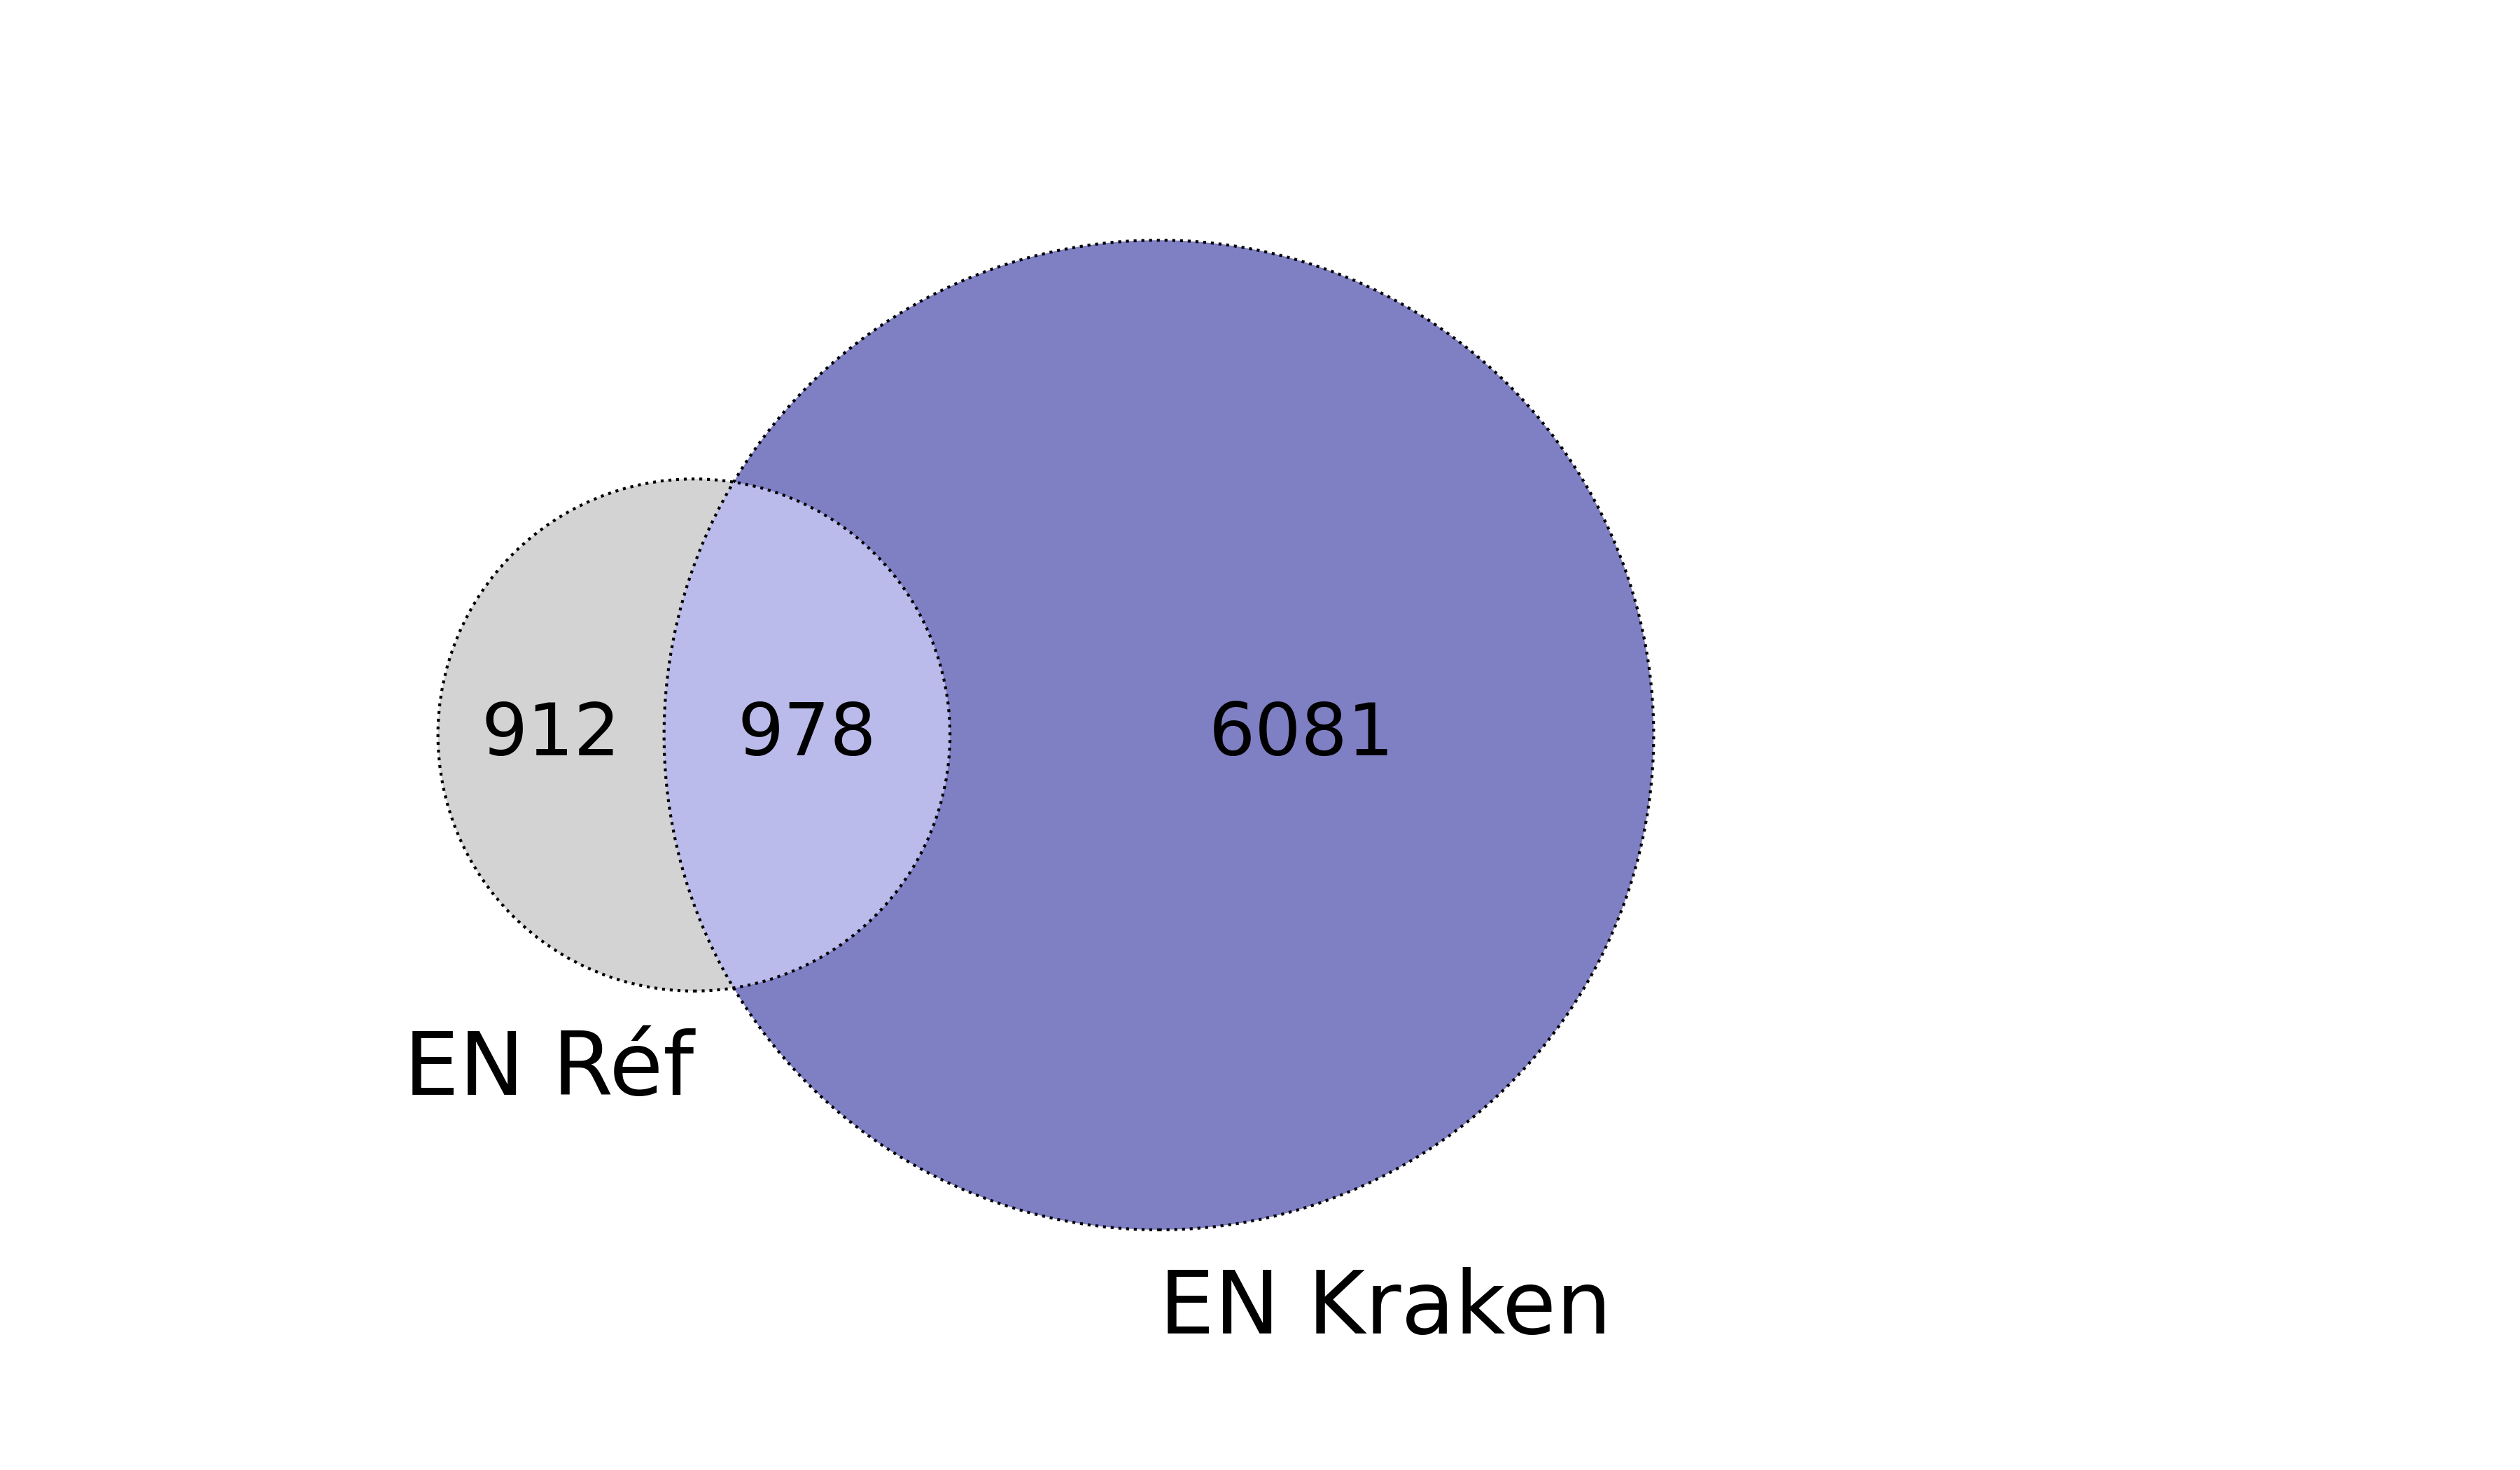
\includegraphics[width=1\textwidth]{IMAGES/INTERSECTIONS_GLOBALES/ELTeCFRA_Kraken_spacy-lg-concat_intersection.png} 
  \caption{Kraken --\texttt{spaCy-lg}}
  \label{fig:ELTeCFRA_Kraken_spacy-lg-concat_intersection}
  \end{subfigure}
  \end{minipage}
  \begin{minipage}{7cm}
  \begin{subfigure}{1\textwidth}
%  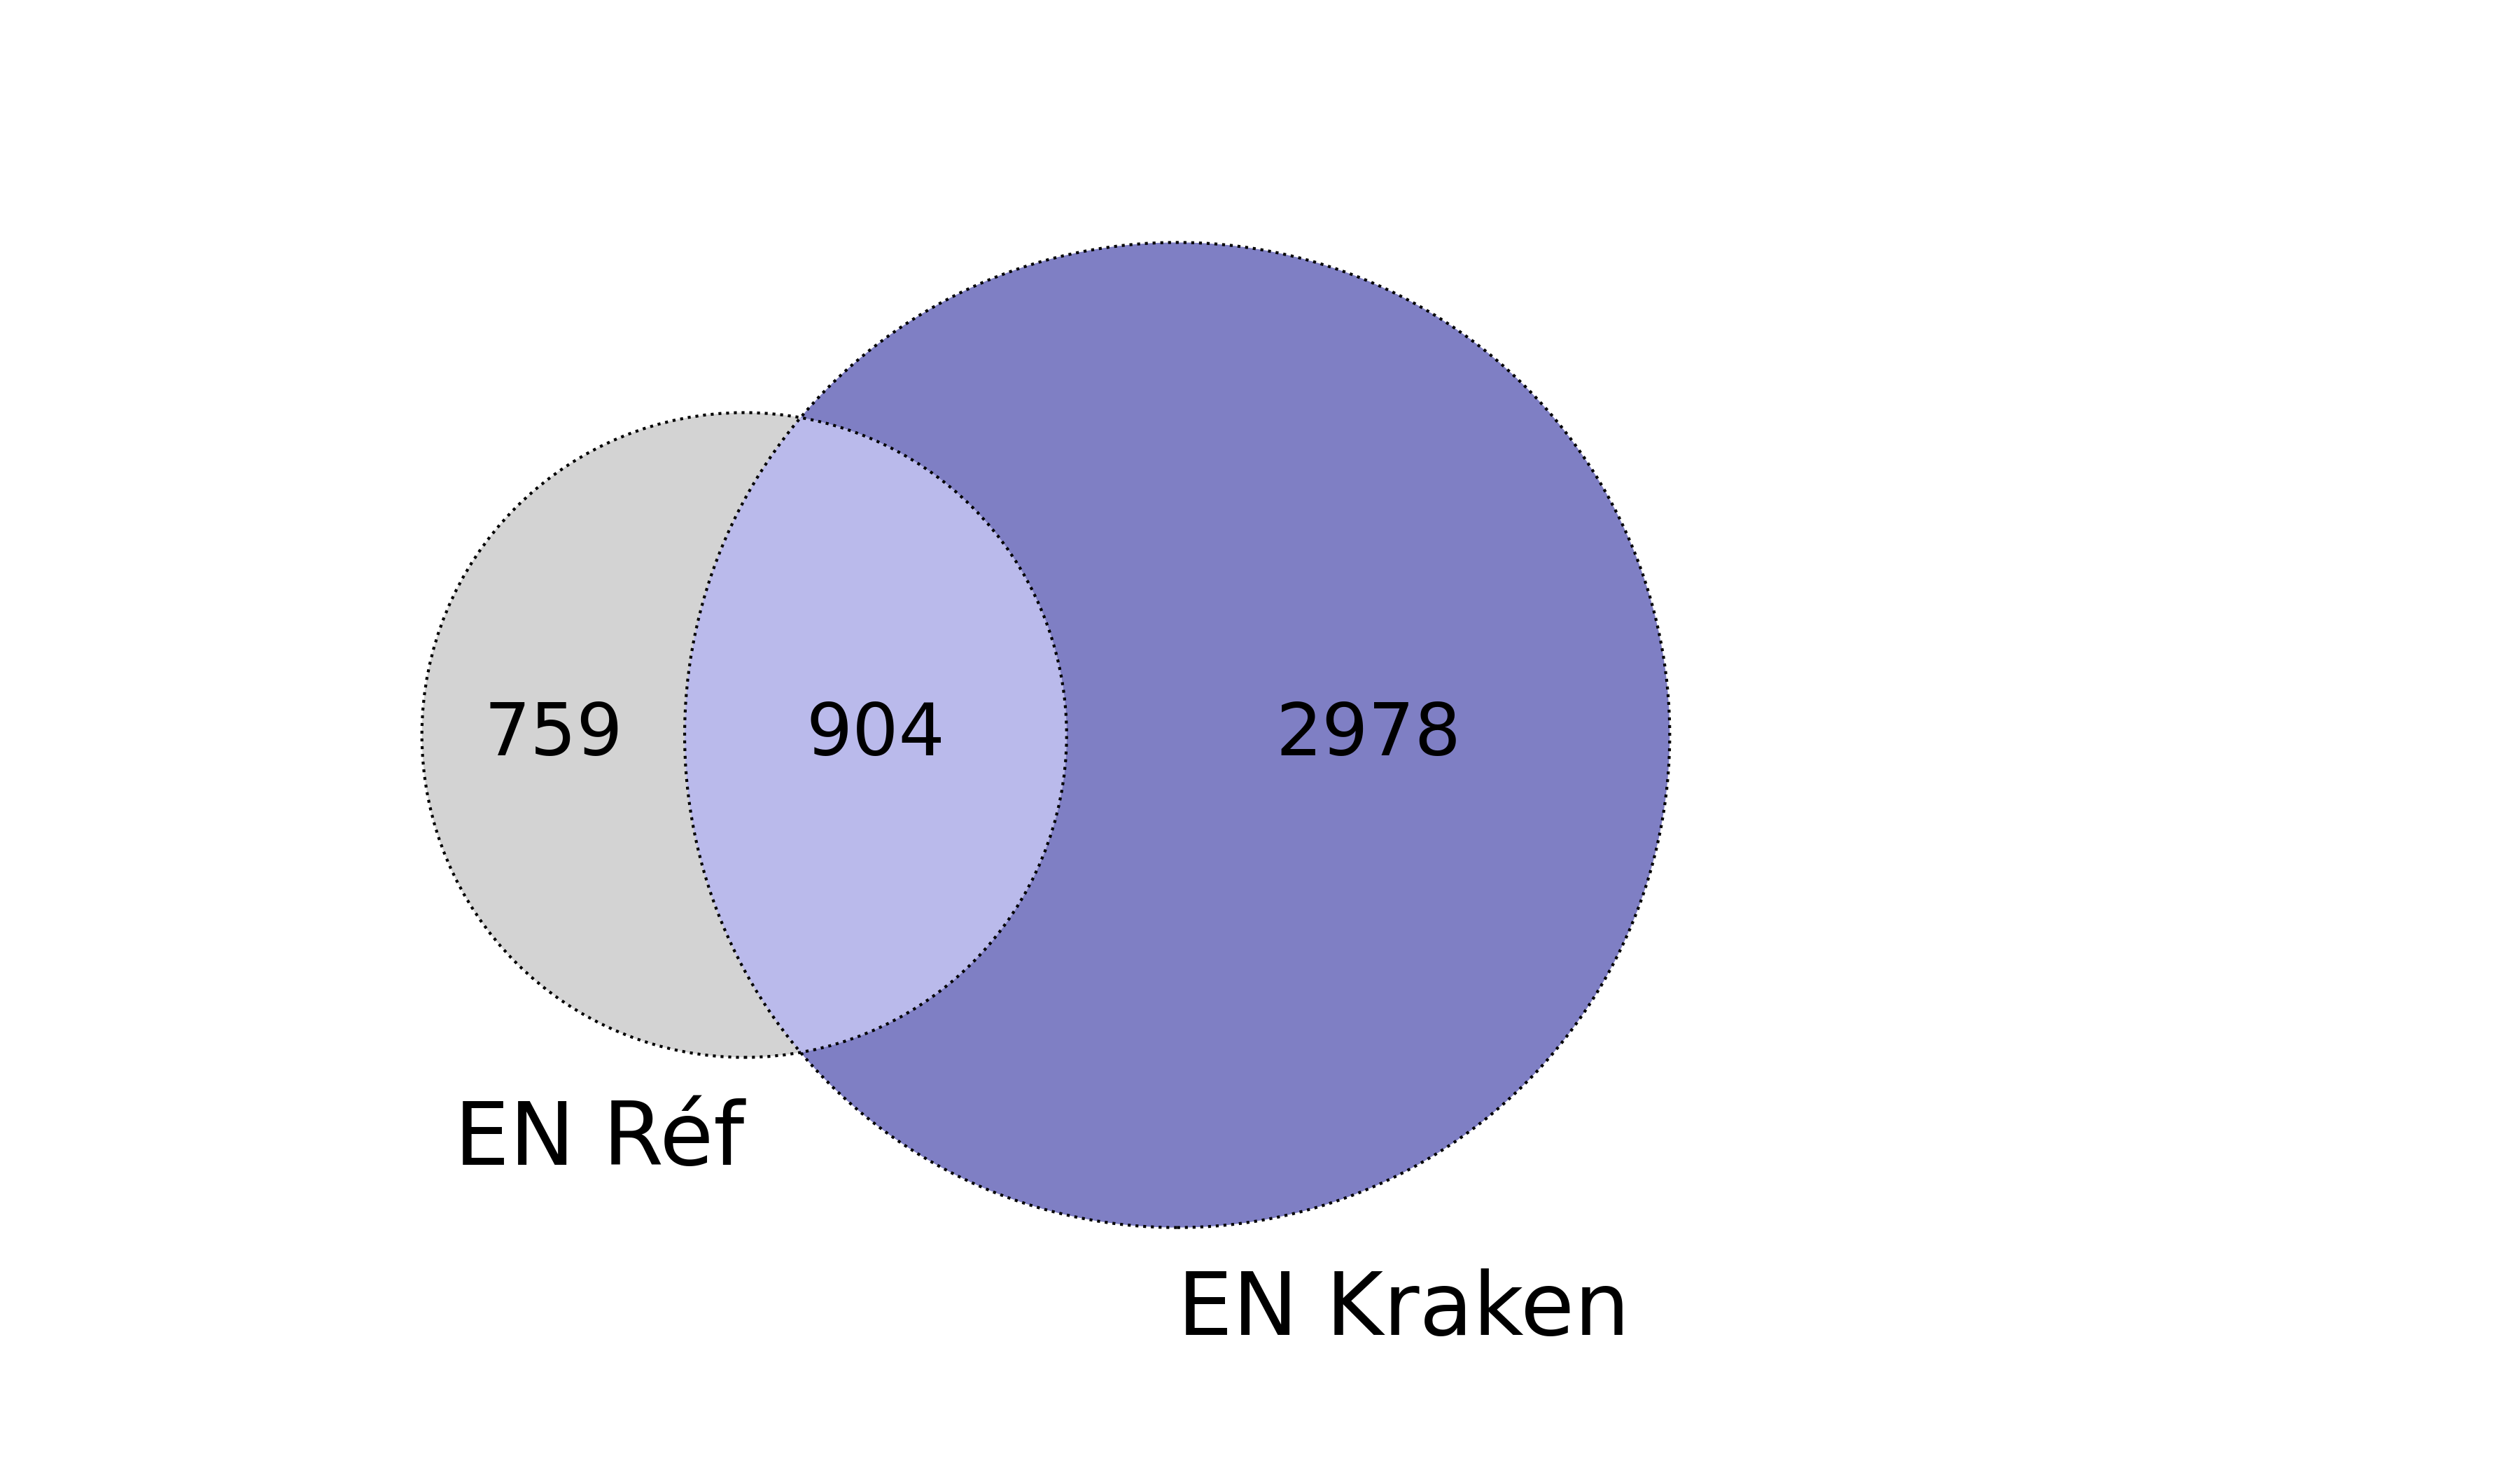
\includegraphics[width=1\textwidth]{IMAGES/INTERSECTIONS_GLOBALES/ELTeCFRA_Kraken_stanza-concat_intersection.png} %%%% ancienne figure 07/02/2024
  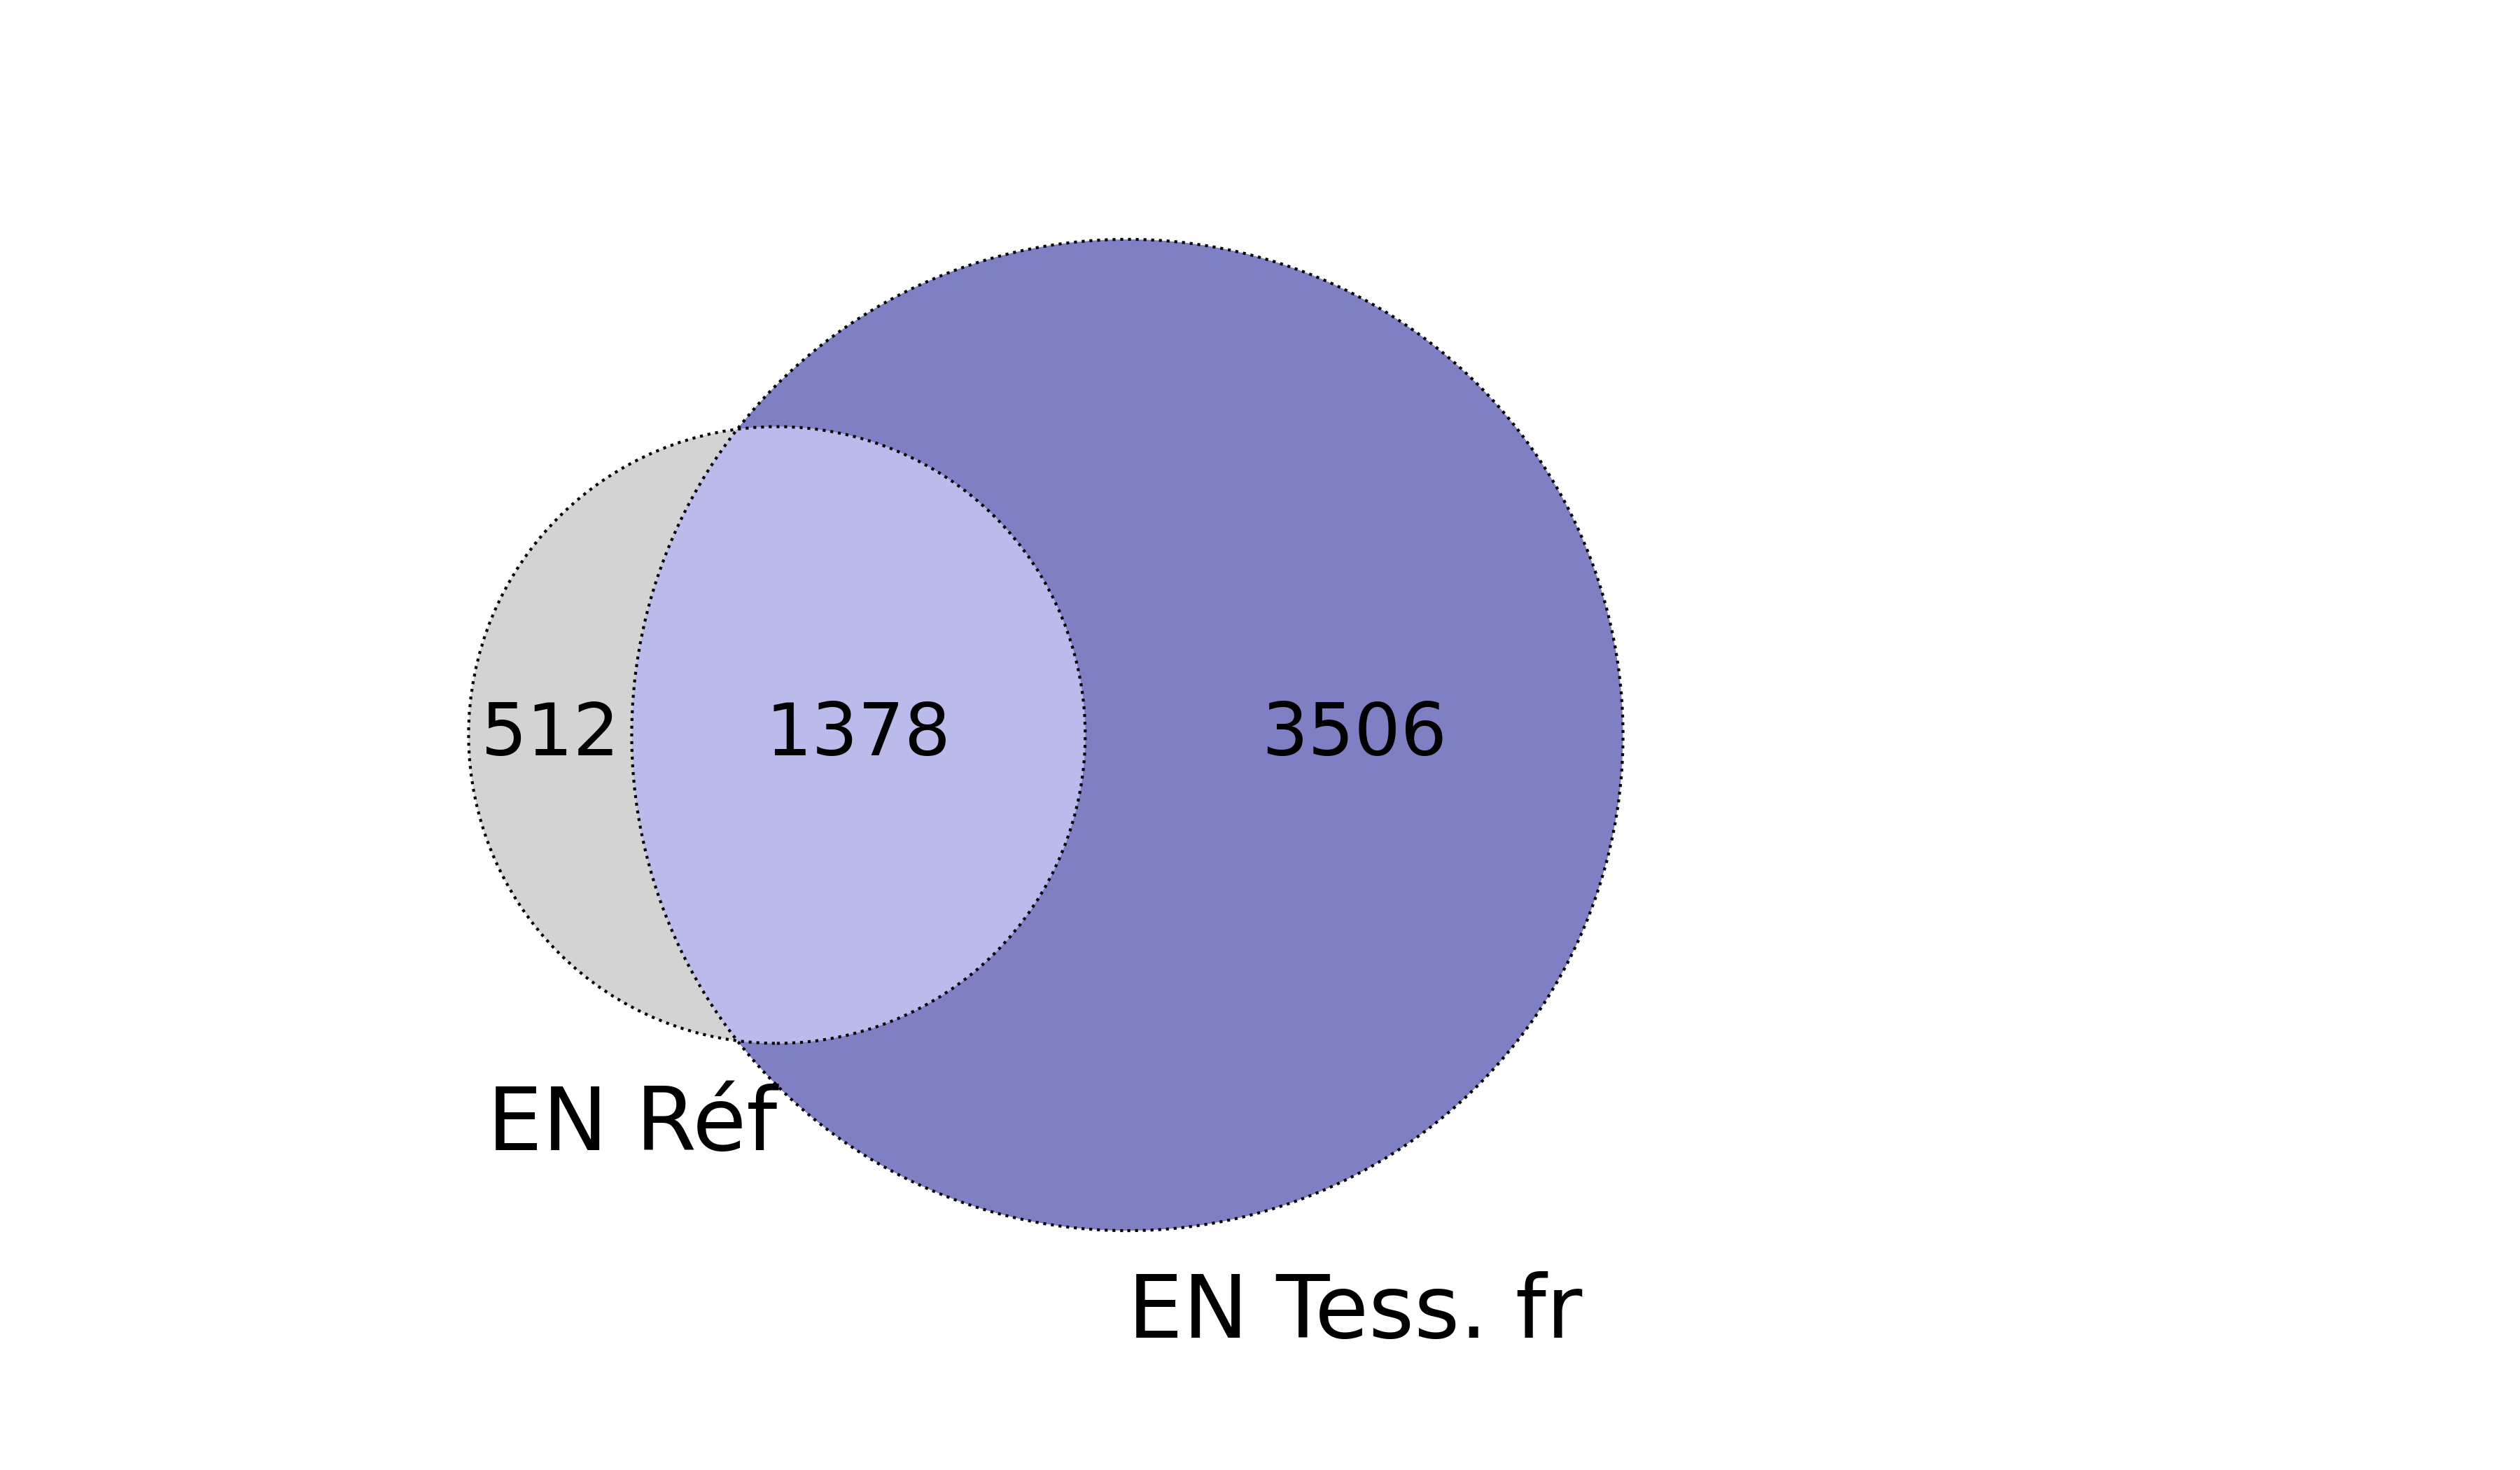
\includegraphics[width=1\textwidth]{IMAGES/INTERSECTIONS_GLOBALES/ELTeCFRA_Tess. fr_spacy-lg-concat_intersection.png}
  \caption{Tess. fr. -- \texttt{spaCy\_lg}}
 % \label{fig:ELTeCFRA_Kraken_stanza-concat_intersection}
  \end{subfigure}
    \end{minipage}
%\begin{minipage}{7cm}
%  \begin{subfigure}{1\textwidth}
%  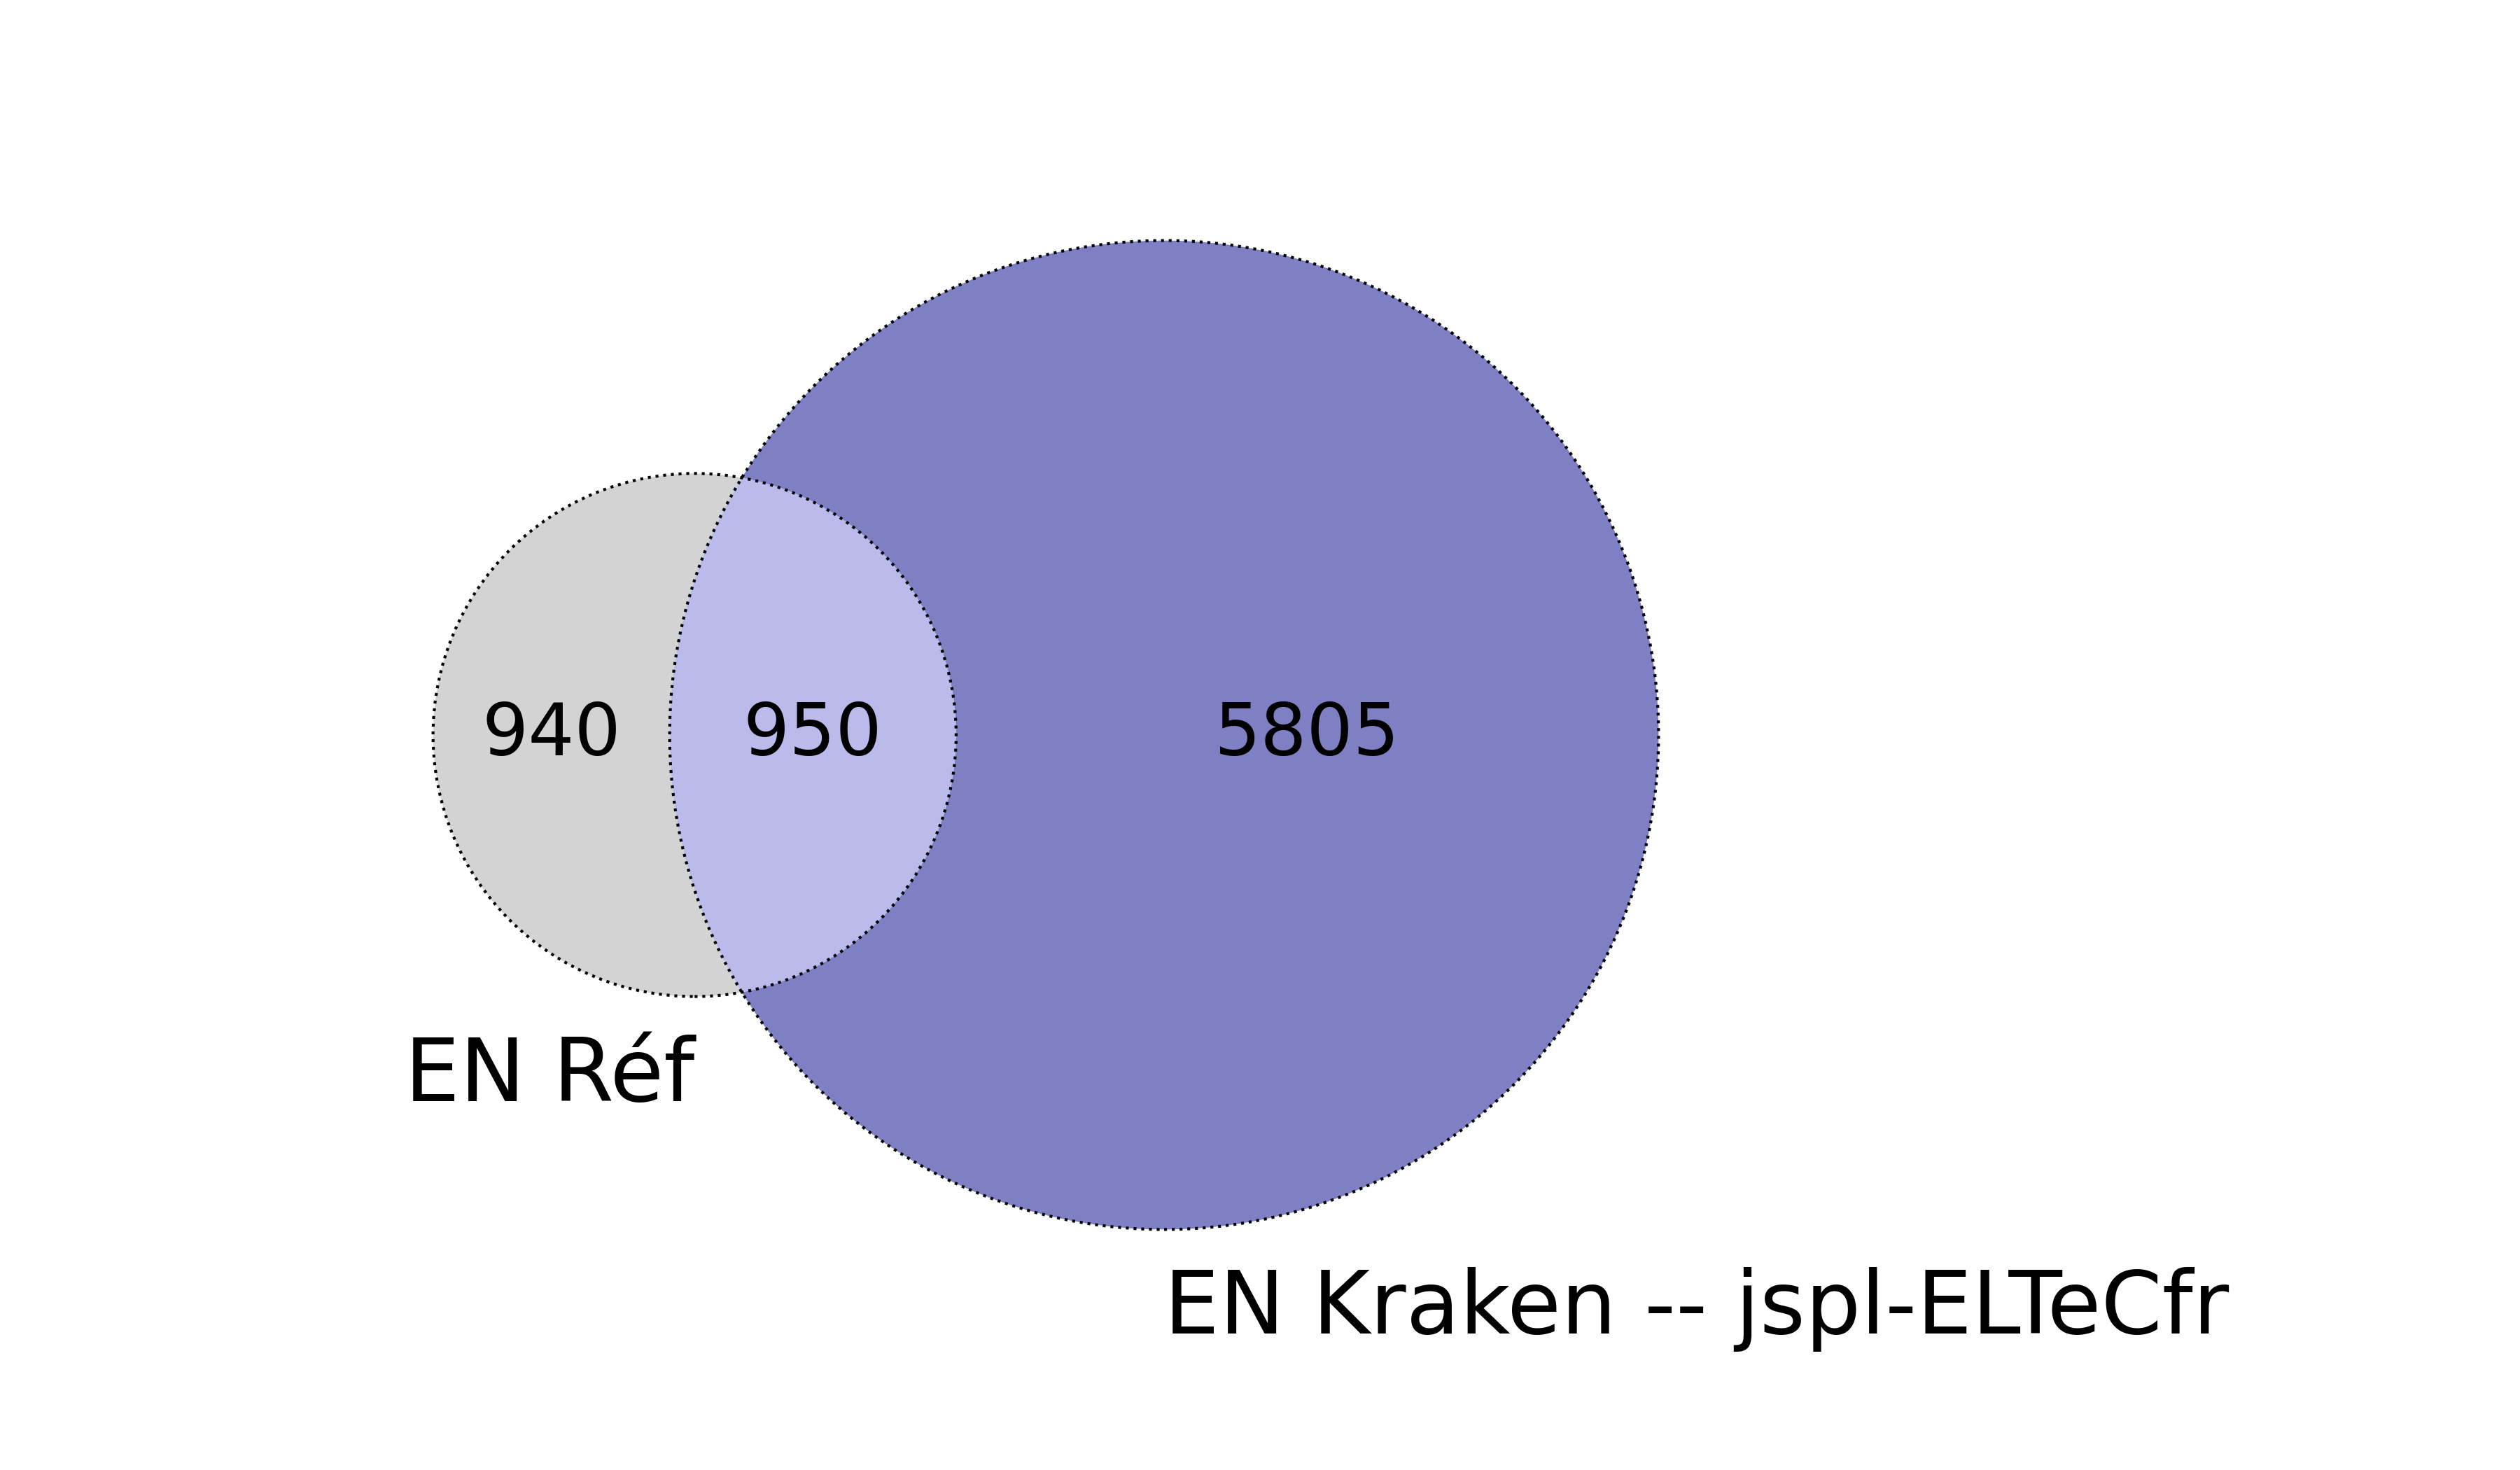
\includegraphics[width=1\textwidth]{IMAGES/INTERSECTIONS_GLOBALES/ELTeCFRA_Kraken -- jspl-ELTeCfr_spacy-lg-concat_intersection.png} 
%  \caption{Kraken corrigé ELTeC-fr -- \texttt{spaCy-lg}}
%  \label{fig:ELTeCFRA_Kraken -- jspl-ELTeCfr_spacy-lg-concat_intersection}
%  \end{subfigure}
%  \end{minipage}
%  \begin{minipage}{7cm}
%  \begin{subfigure}{1\textwidth}
%  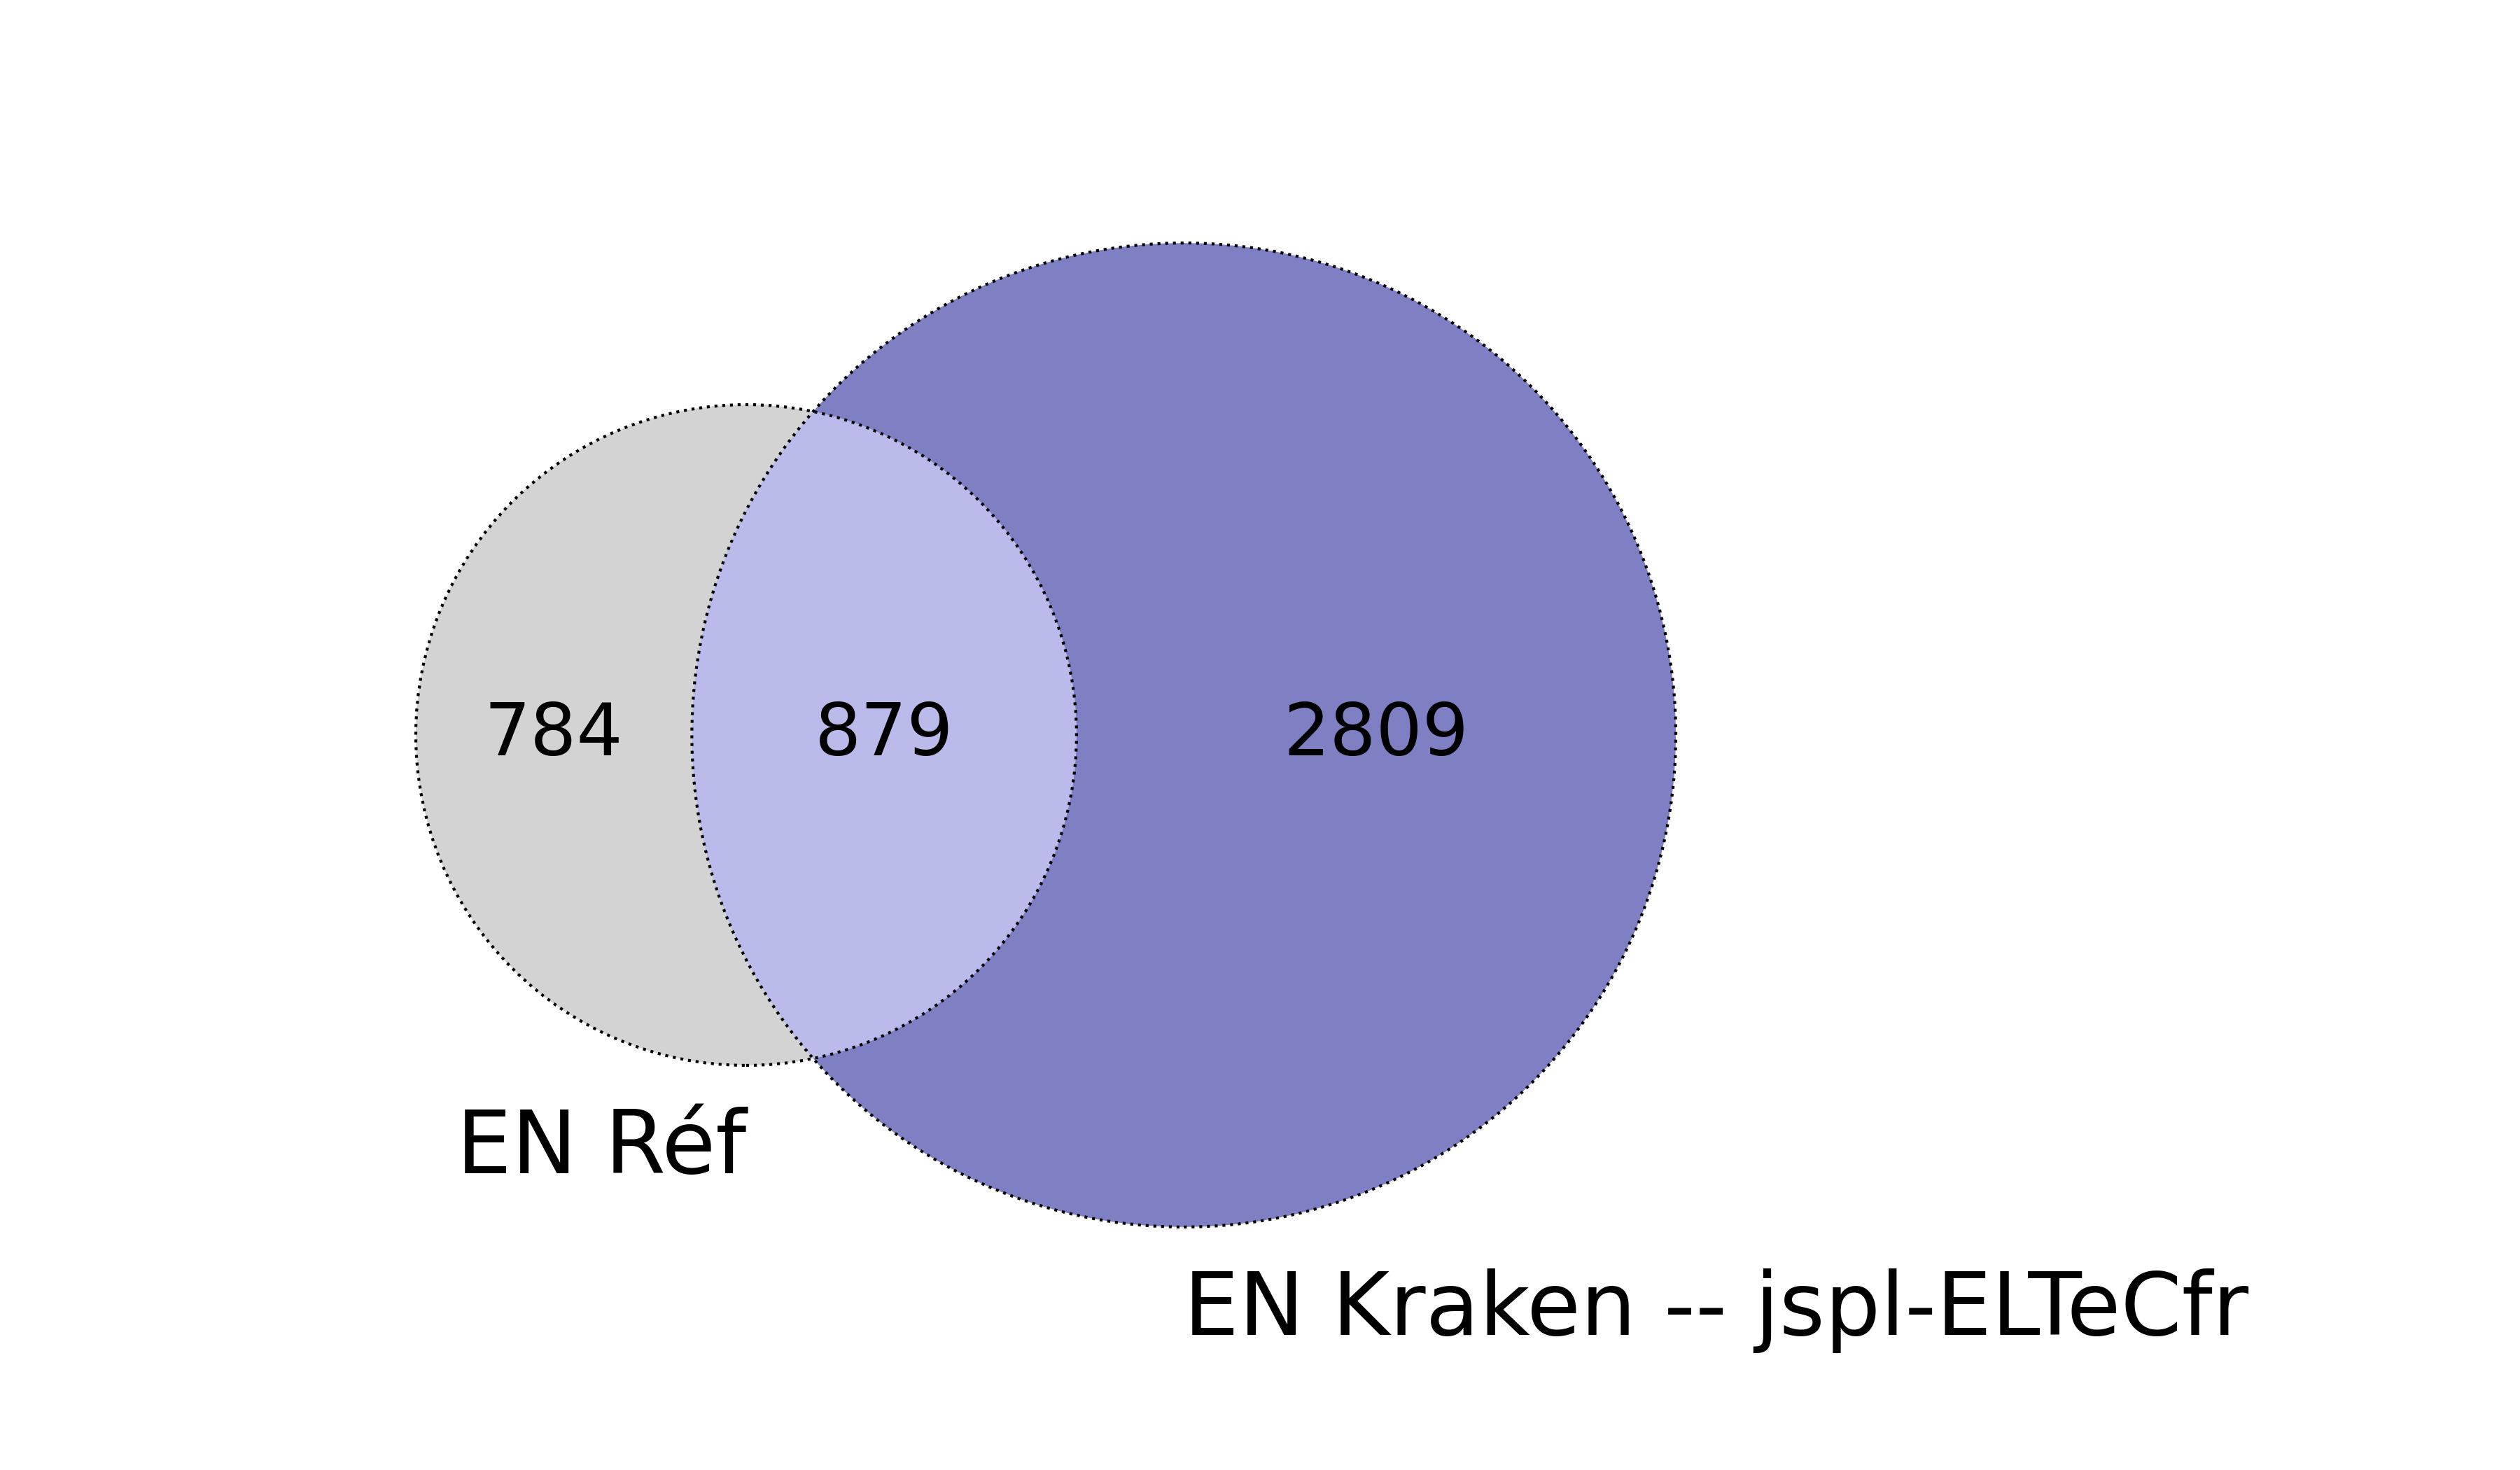
\includegraphics[width=1\textwidth]{IMAGES/INTERSECTIONS_GLOBALES/ELTeCFRA_Kraken -- jspl-ELTeCfr_stanza-concat_intersection.png}
%  \caption{Kraken corrigé ELTeC-fr -- \texttt{stanza}}
%  \label{fig:ELTeCFRA_Kraken -- jspl-ELTeCFR_stanza-concat_intersection}
%  \end{subfigure}
%    \end{minipage}
\caption{Intersections pour les configurations Kraken-\texttt{spaCy\_lg} et Tess. fr.-\texttt{spaCy\_lg}, pour le sous-corpus ELTeC français.}
%\label{fig:intersection_globale-kraken}
\label{fig:intersection_globale-kraken-tess}
\end{figure}

%%%%%%%%%%%% ancienne sous-figure 07/02/2024
%\begin{figure}[h!]
%    \begin{minipage}{7cm}
%  \begin{subfigure}{1\textwidth}
%  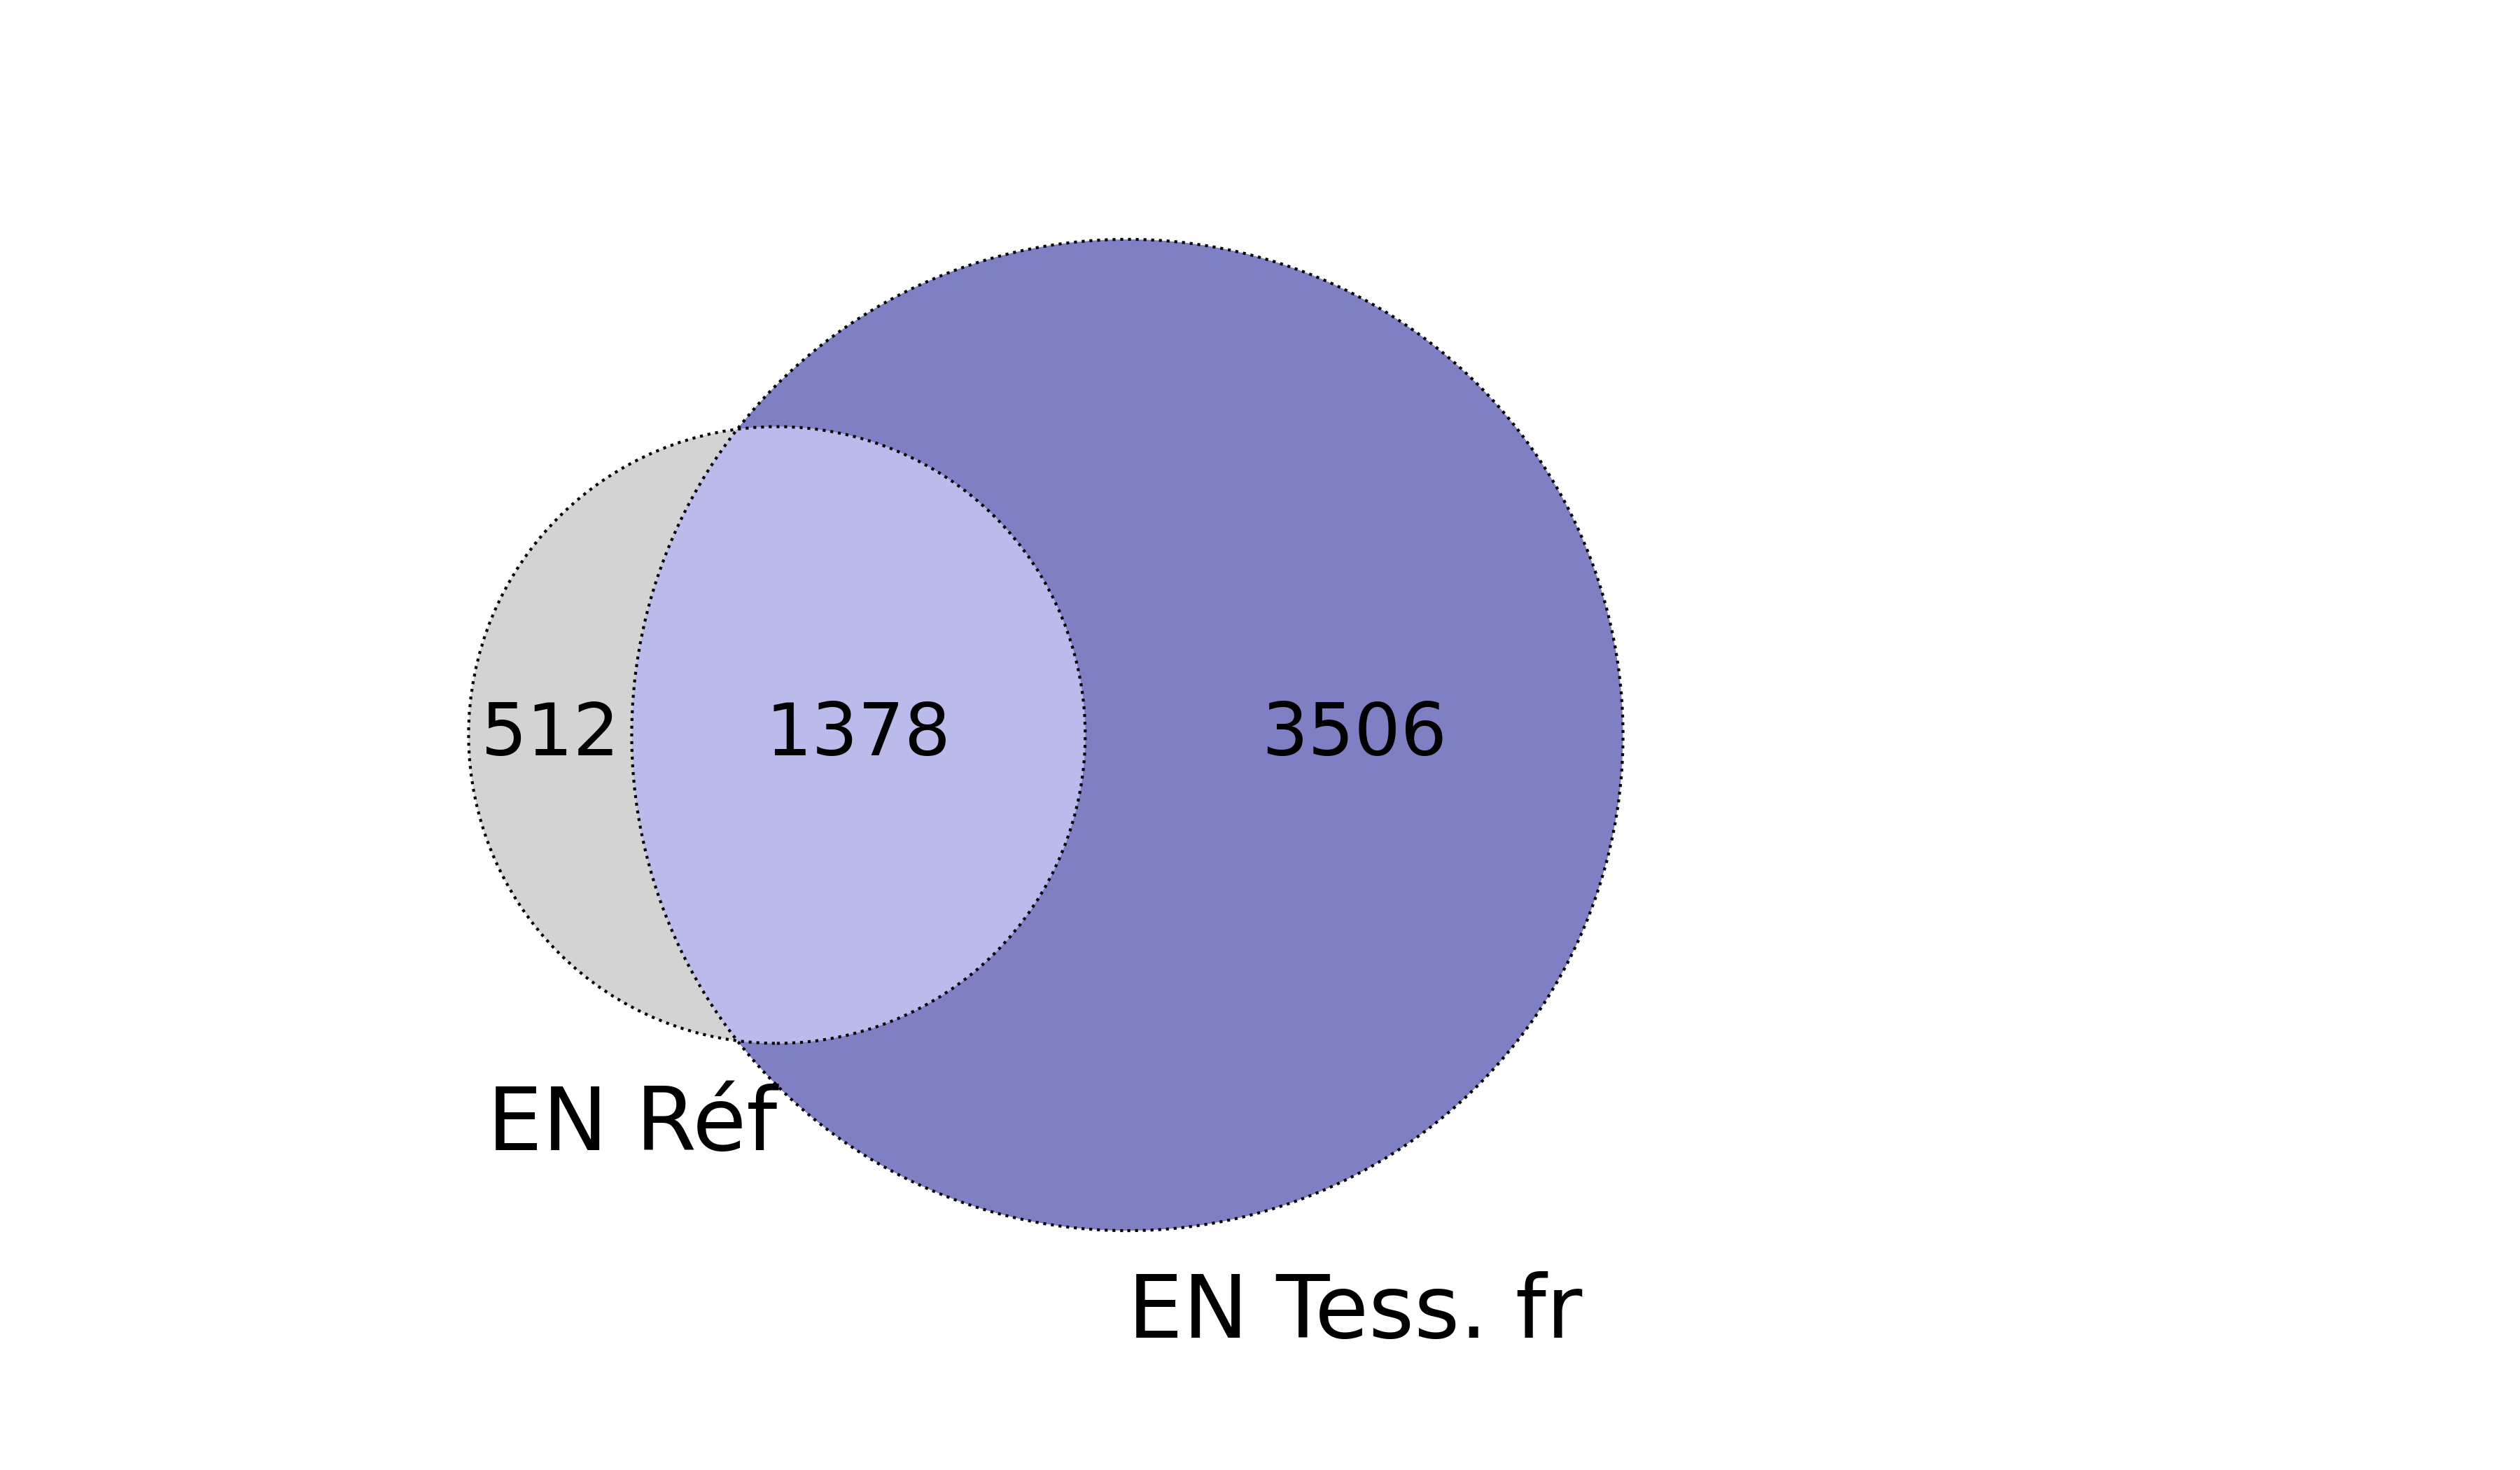
\includegraphics[width=1\textwidth]{IMAGES/INTERSECTIONS_GLOBALES/ELTeCFRA_Tess. fr_spacy-lg-concat_intersection.png} 
%  \caption{Tess. fr. --\texttt{spaCy\_lg}}
%  \label{fig:ELTeCFRA_Tess. fr_spacy-lg-concat_intersection}
%  \end{subfigure}
%  \end{minipage}
%  \begin{minipage}{7cm}
%  \begin{subfigure}{1\textwidth}
%  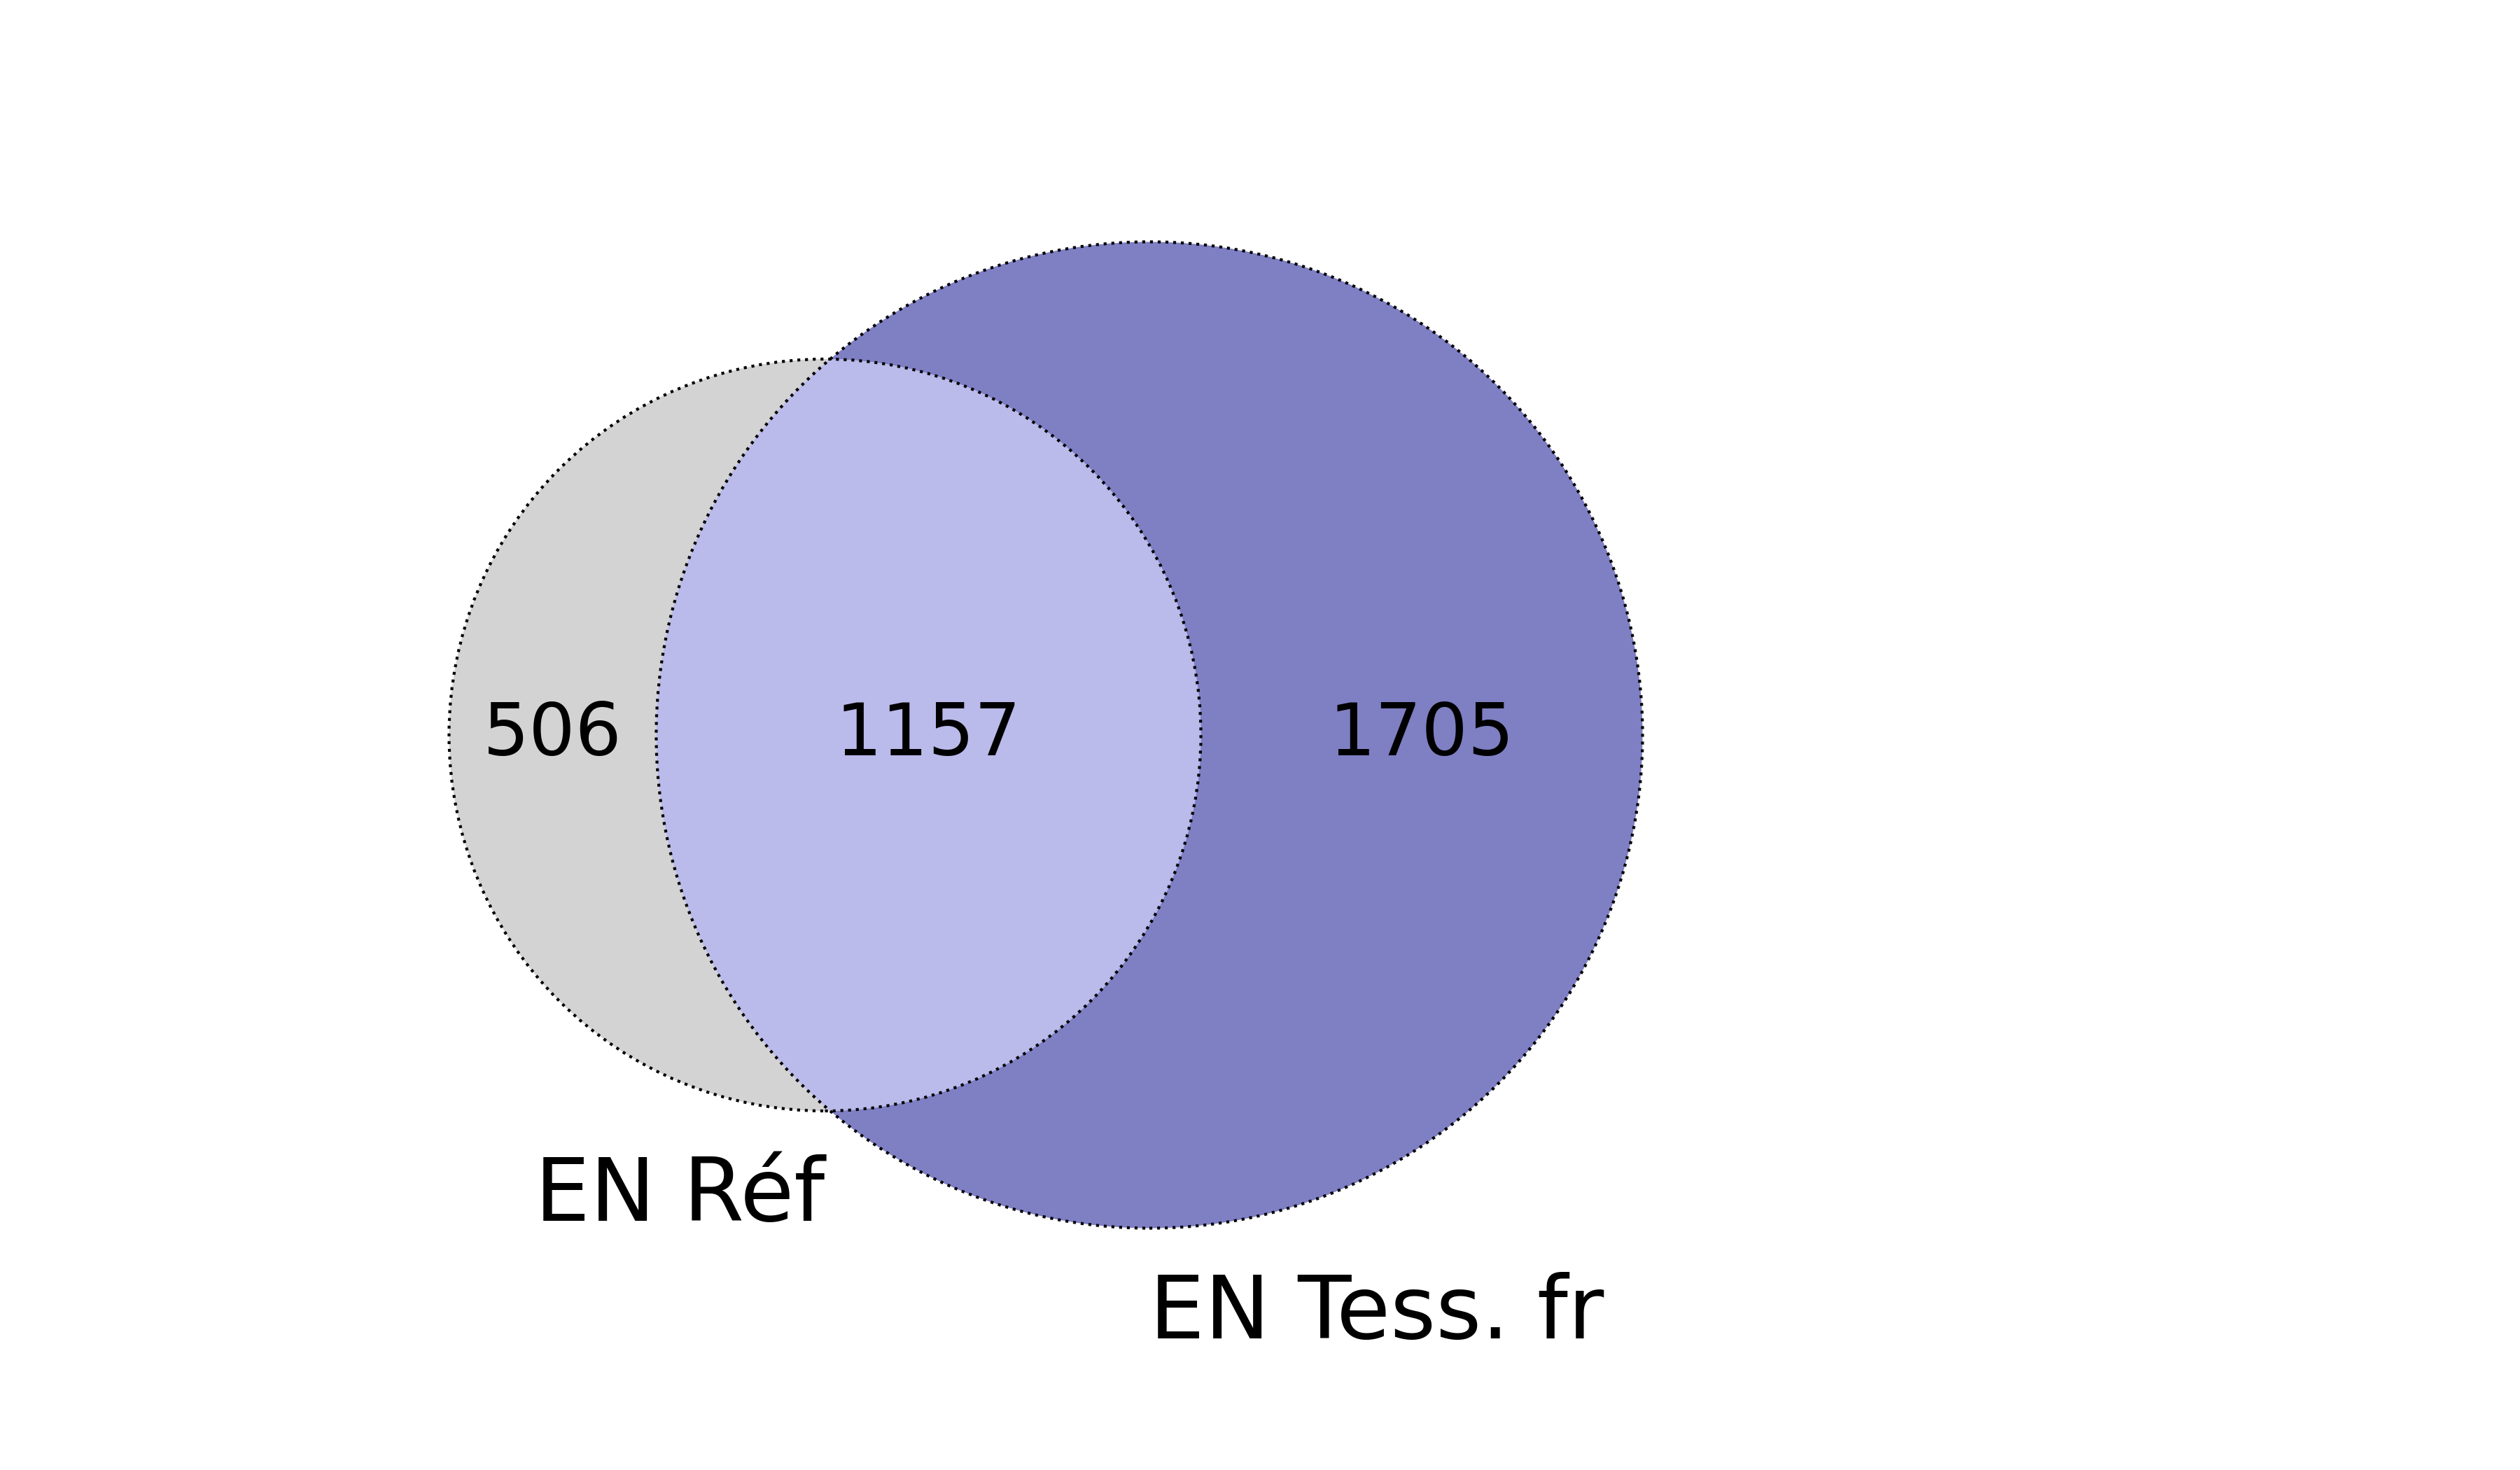
\includegraphics[width=1\textwidth]{IMAGES/INTERSECTIONS_GLOBALES/ELTeCFRA_Tess. fr_stanza-concat_intersection.png}
%  \caption{Tess. fr. -- \texttt{stanza}}
% % \label{fig:ELTeCFRA_Tess. fr_stanza-concat_intersection}
%  \end{subfigure}
%    \end{minipage}

%\begin{minipage}{7cm}
%  \begin{subfigure}{1\textwidth}
%  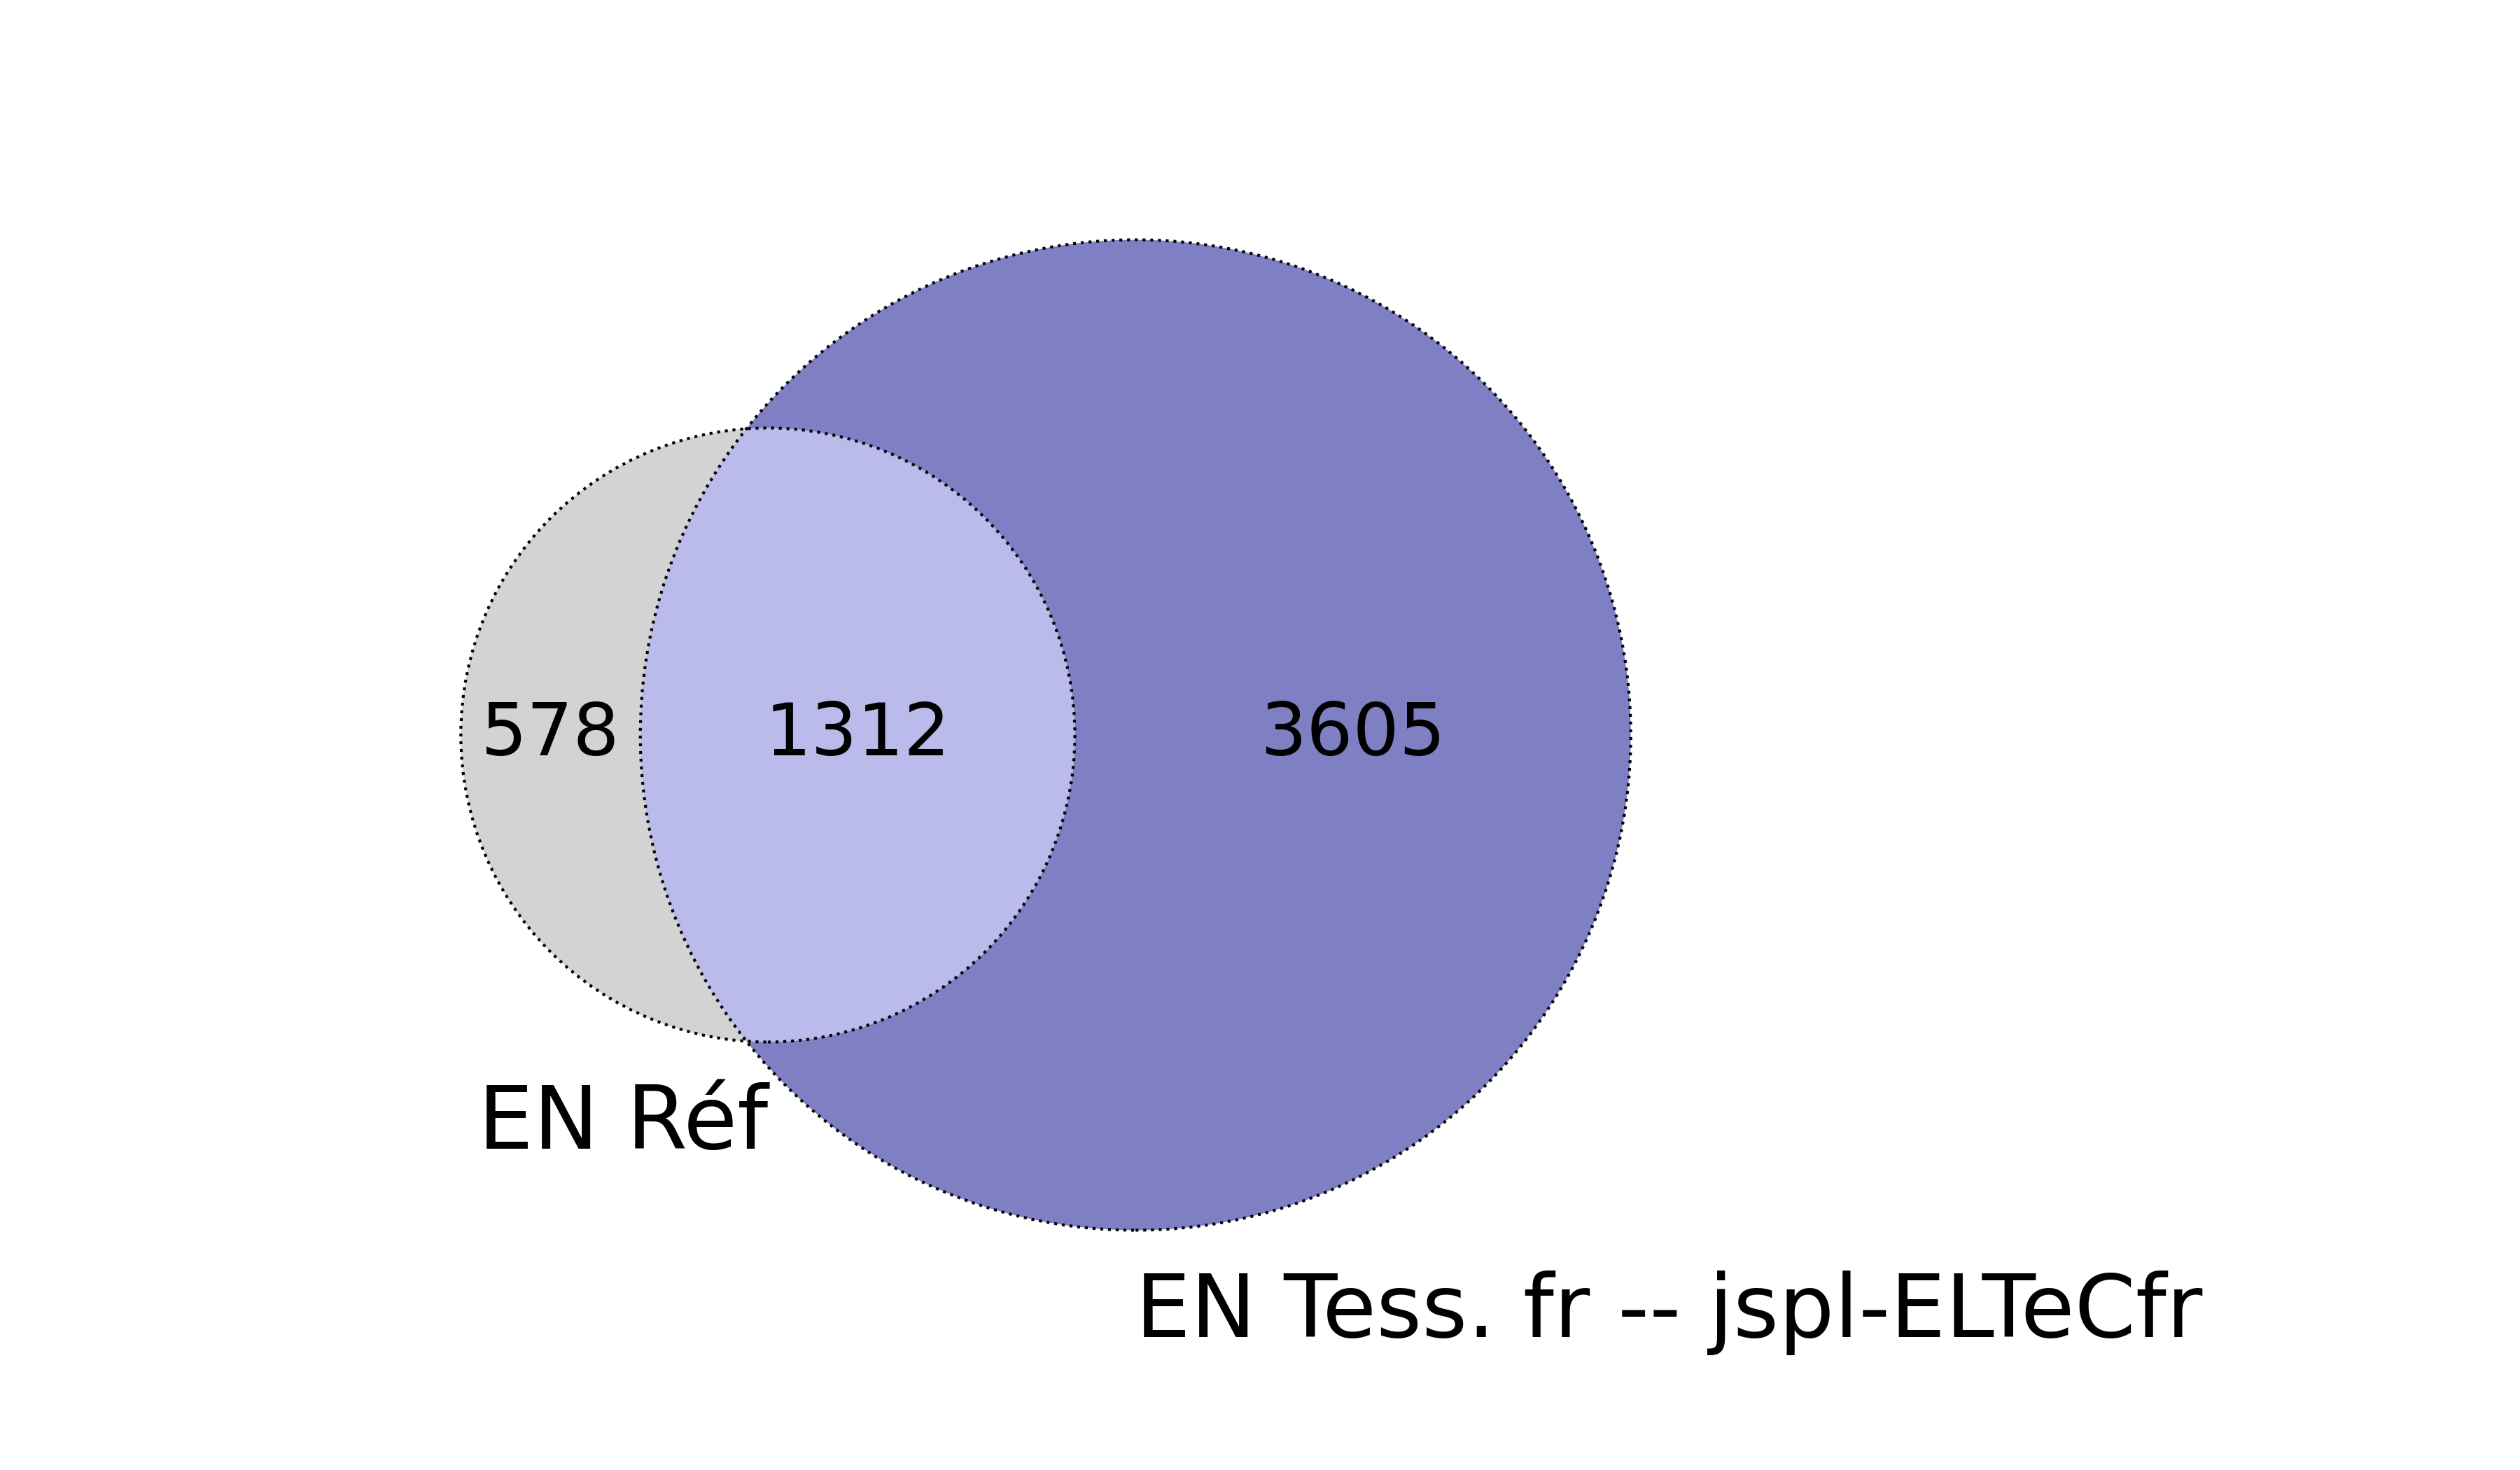
\includegraphics[width=1\textwidth]{IMAGES/INTERSECTIONS_GLOBALES/ELTeCFRA_Tess. fr -- jspl-ELTeCfr_spacy-lg-concat_intersection.png} 
%  \caption{Tess. fr. corrigé -- \texttt{spaCy\_lg}}
%  \label{fig:ELTeCFRA_Tess. fr -- jspl-ELTeCfr_spacy-lg-concat_intersection}
%  \end{subfigure}
% \end{minipage}
%  \begin{minipage}{7cm}
%  \begin{subfigure}{1\textwidth}
%  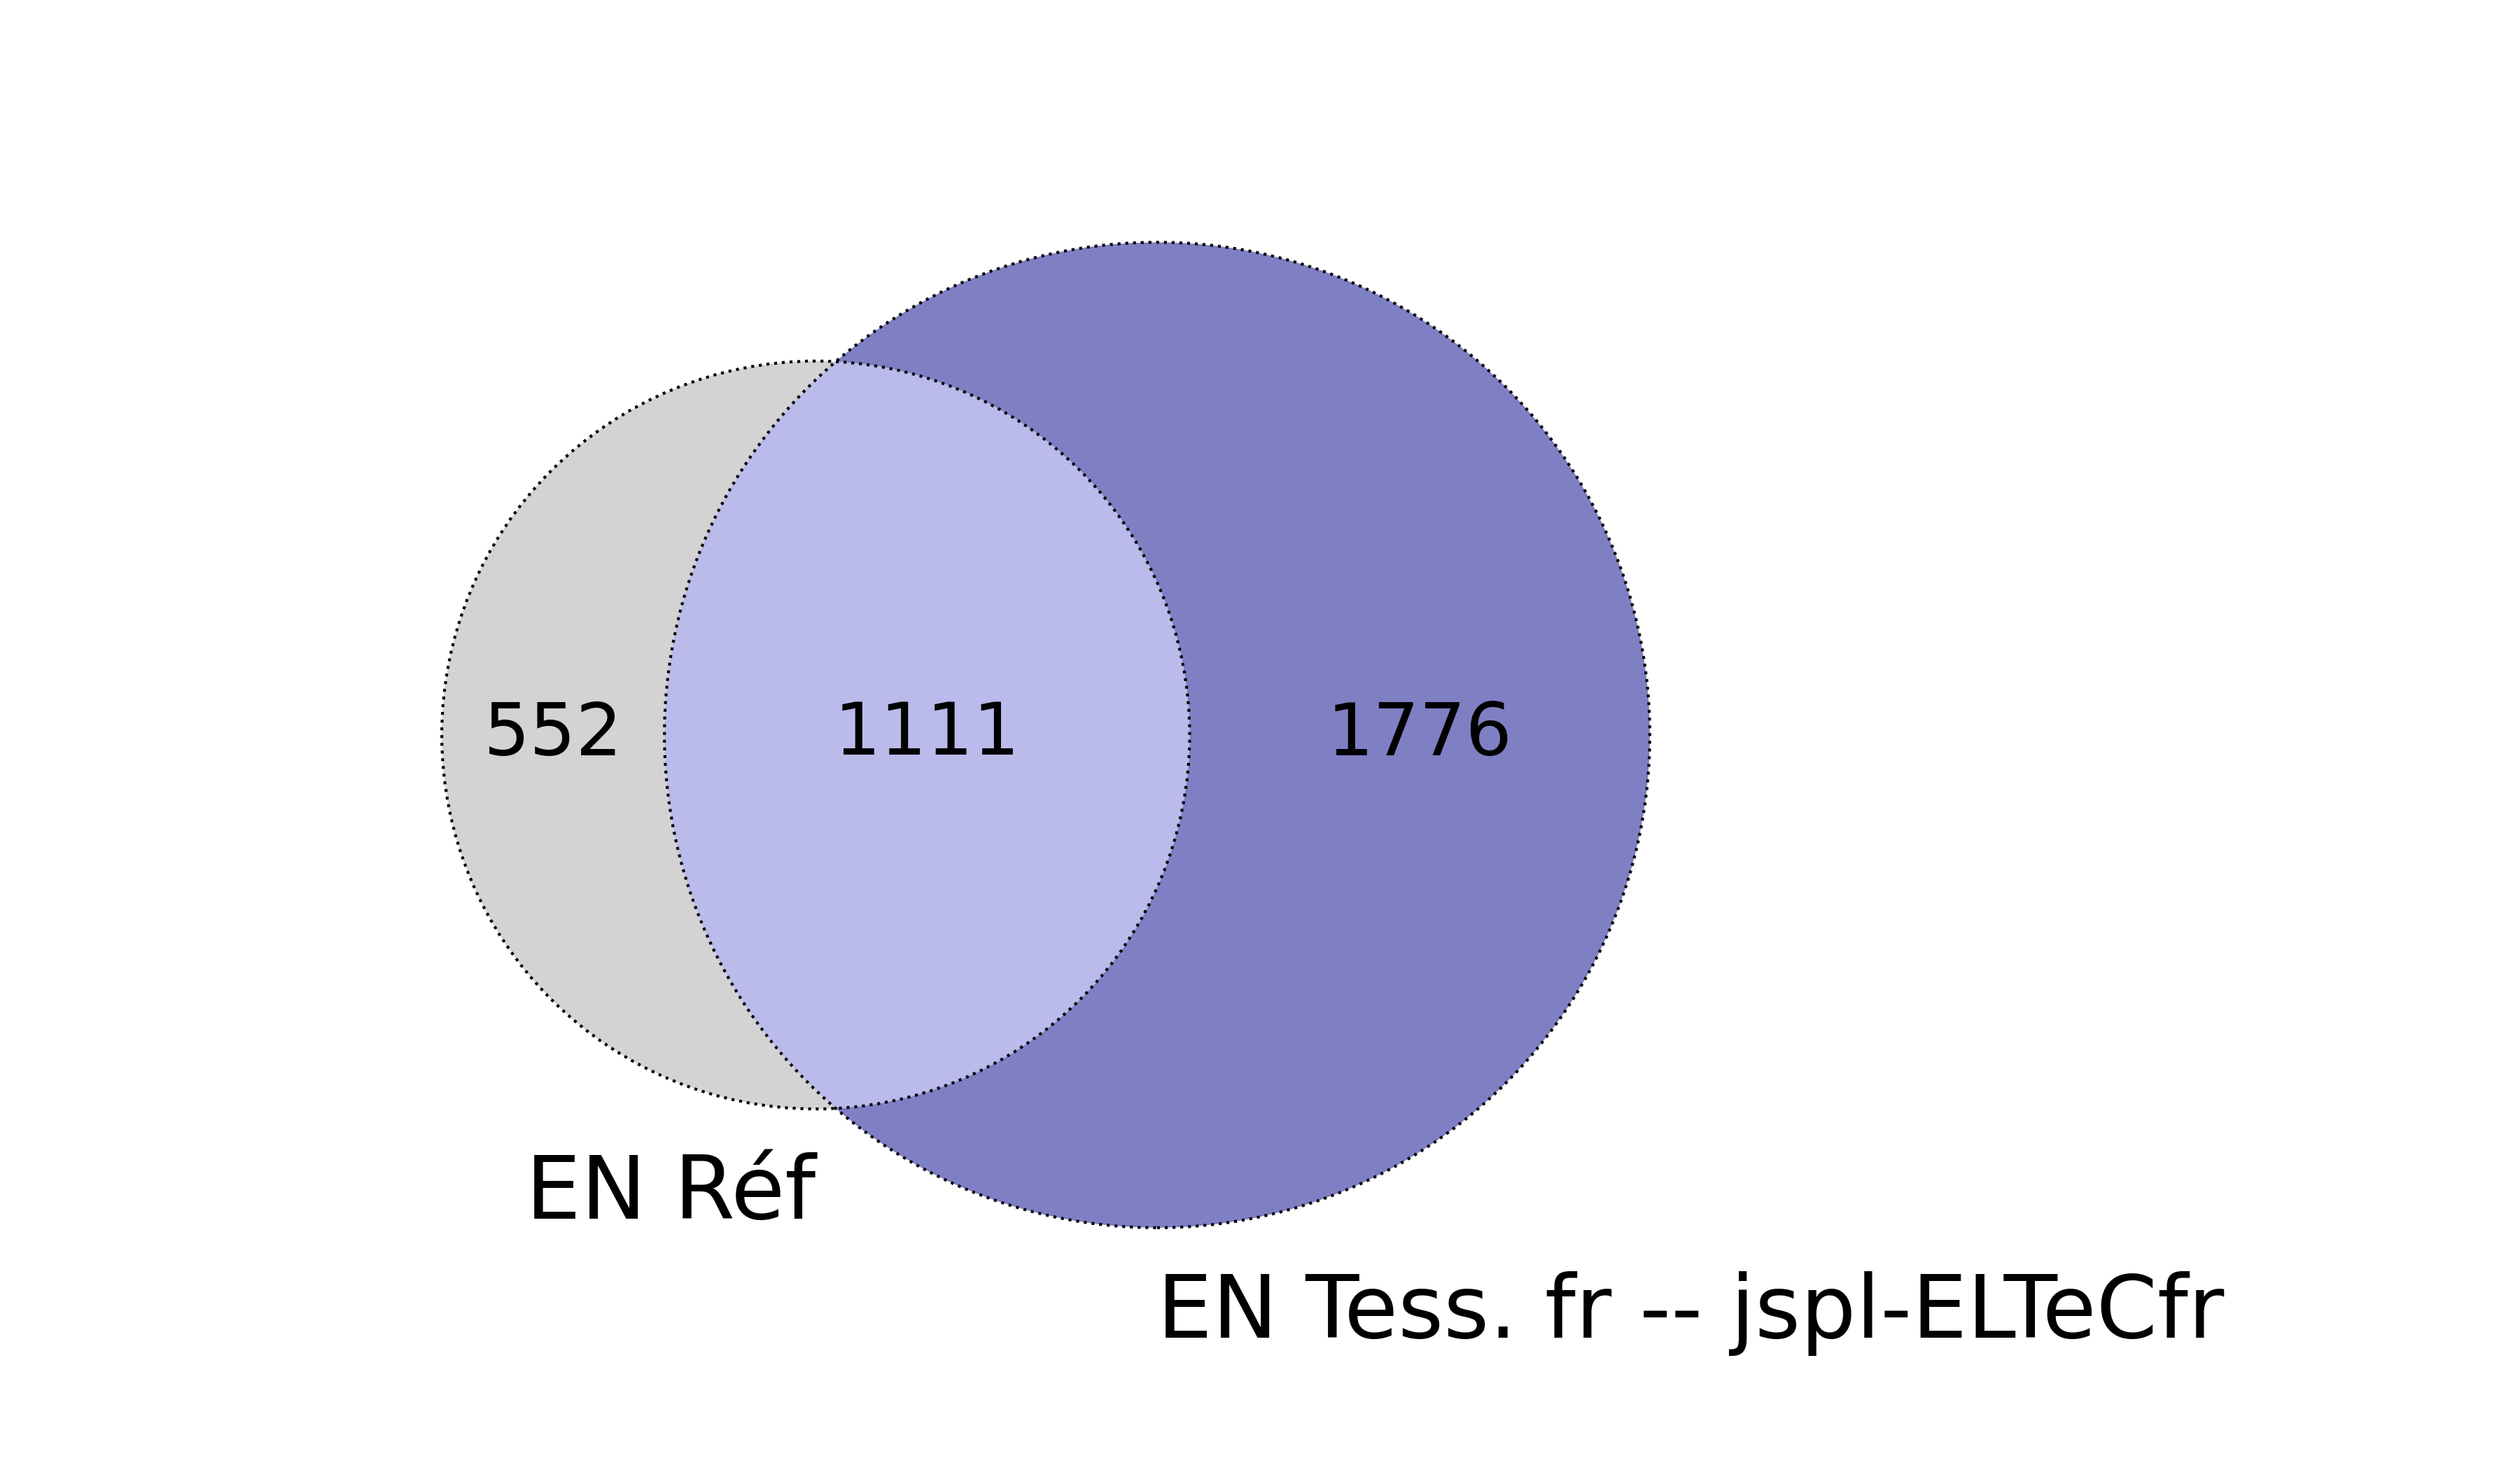
\includegraphics[width=1\textwidth]{IMAGES/INTERSECTIONS_GLOBALES/ELTeCFRA_Tess. fr -- jspl-ELTeCfr_stanza-concat_intersection.png}
%  \caption{Tess. fr. corrigé -- \texttt{stanza}}
%  \label{fig:ELTeCFRA_Tess. fr -- jspl-ELTeCfr_stanza-concat_intersection}
%  \end{subfigure}
%    \end{minipage}
%\begin{minipage}{7cm}
%  \begin{subfigure}{1\textwidth}
%  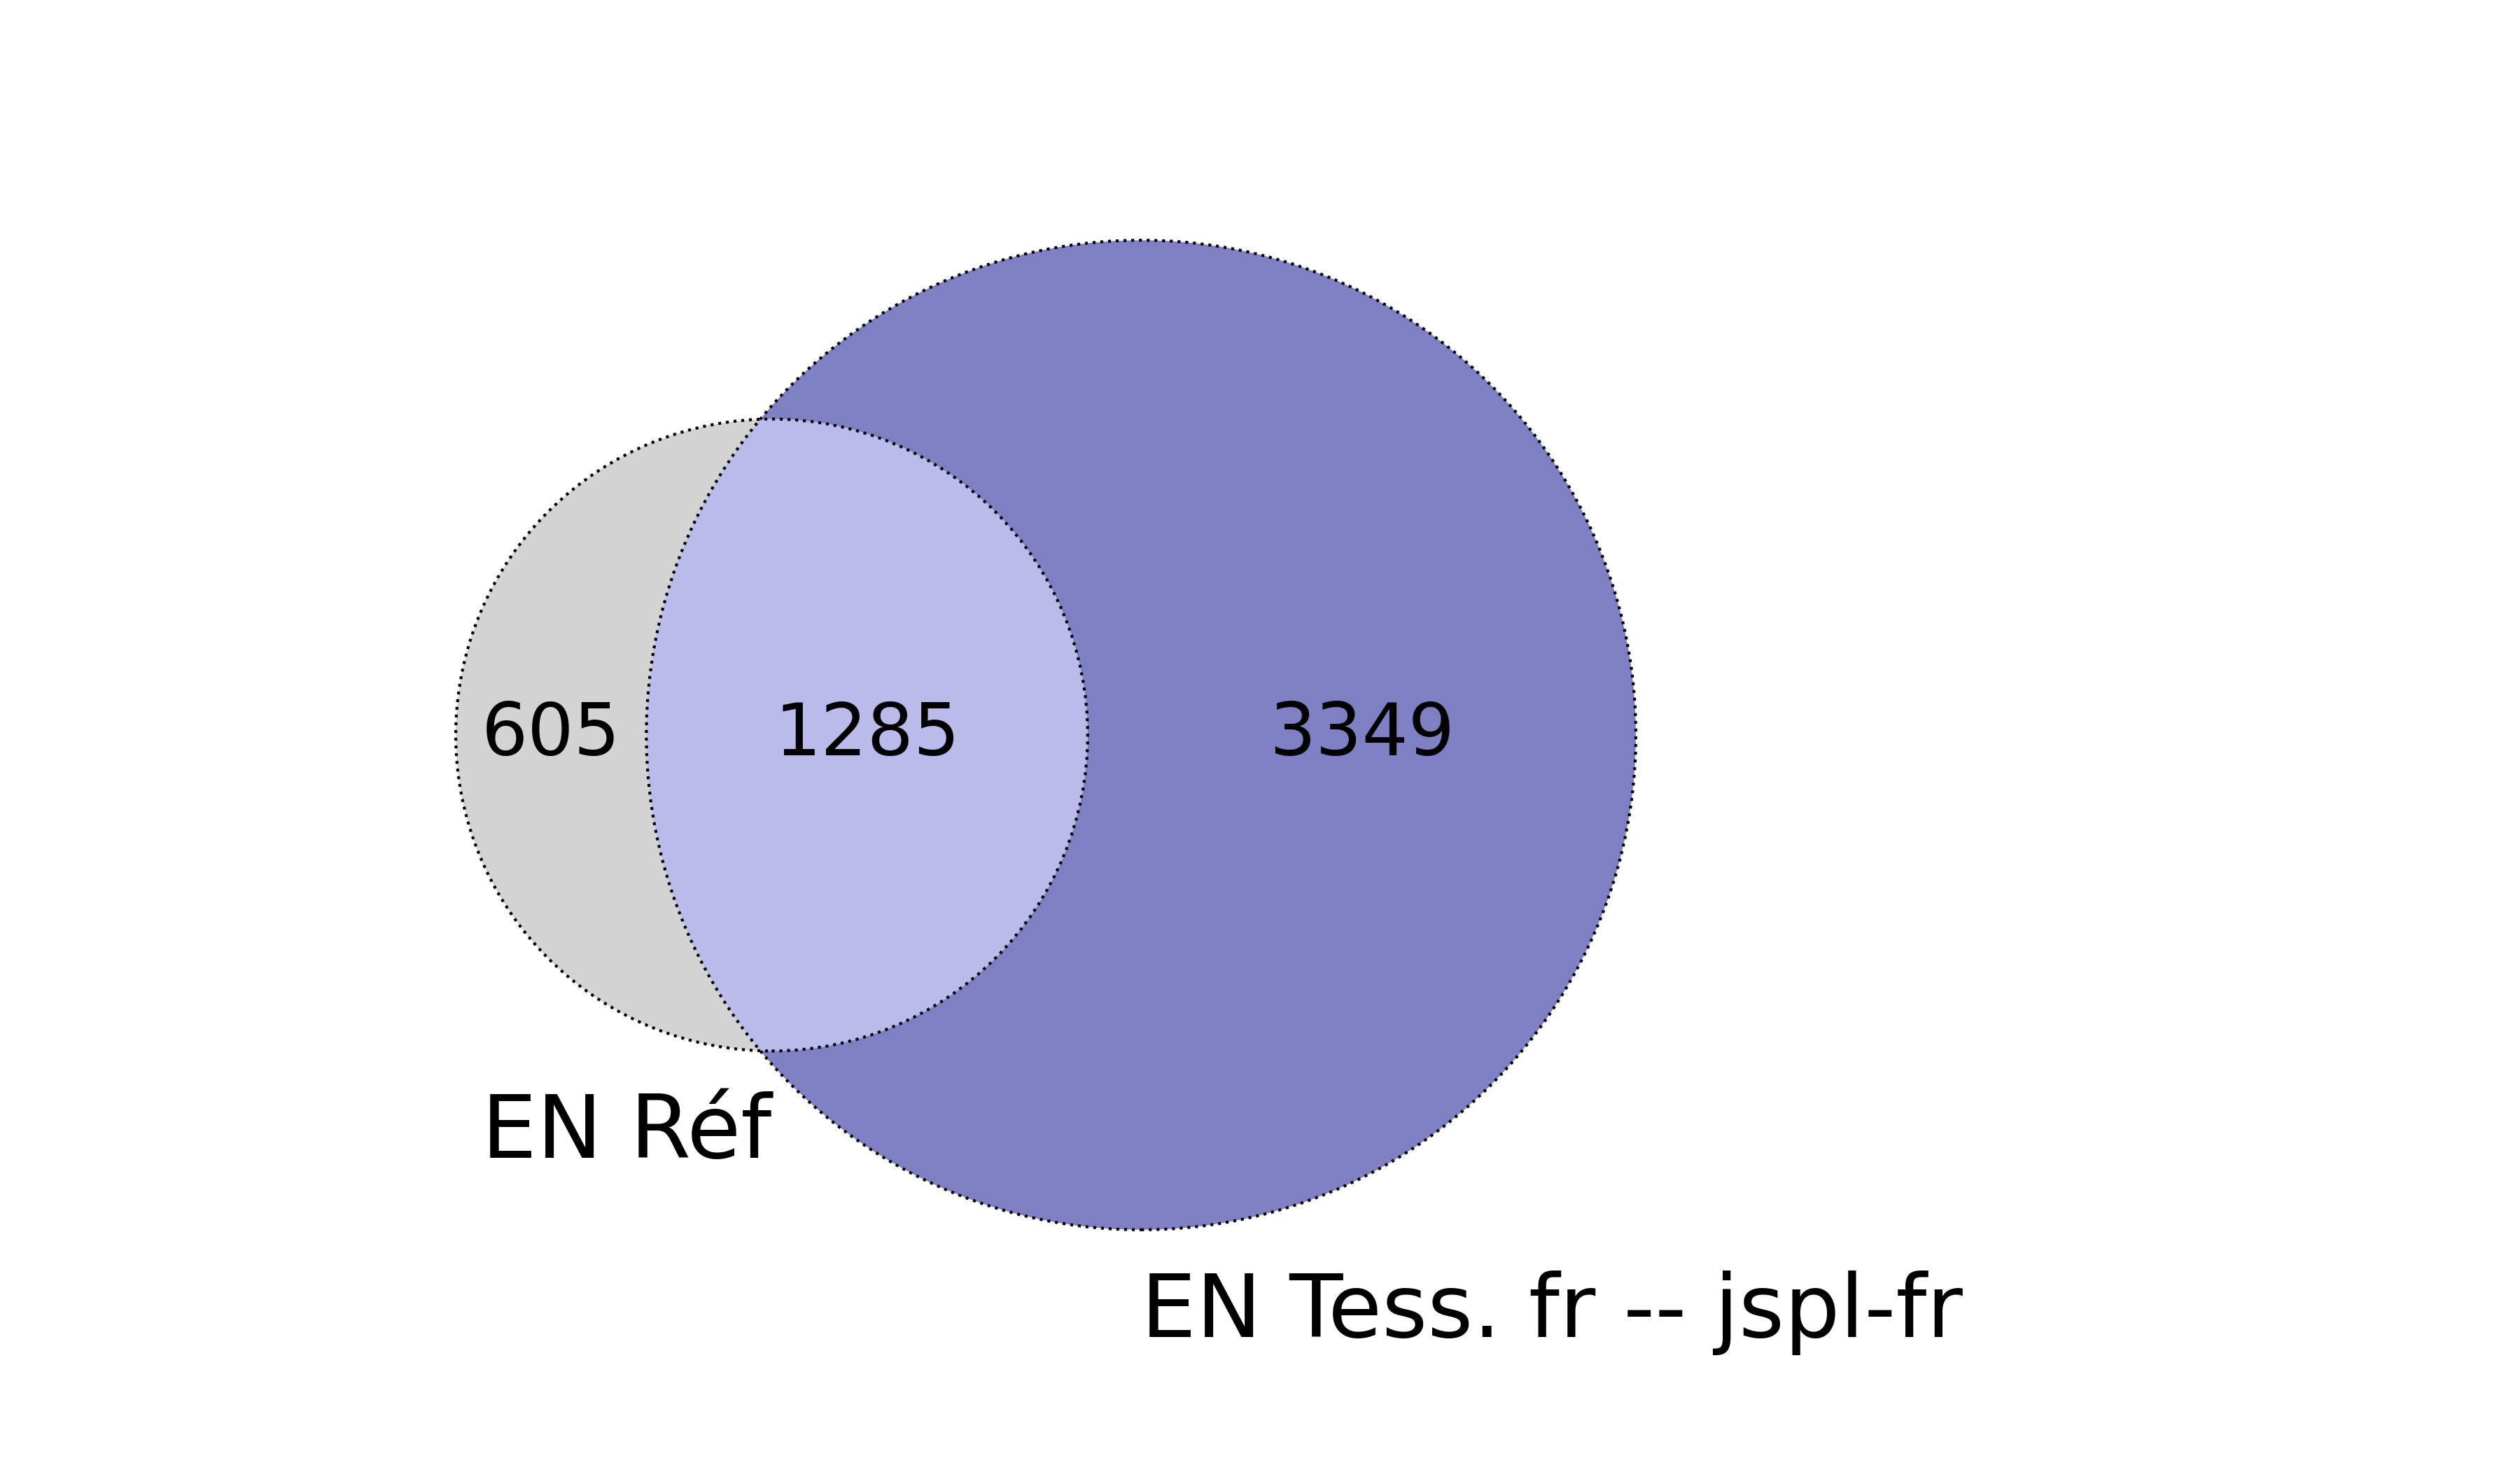
\includegraphics[width=1\textwidth]{IMAGES/INTERSECTIONS_GLOBALES/ELTeCFRA_Tess. fr -- jspl-fr_spacy-lg-concat_intersection.png} 
%  \caption{Tess. fr. corrigé -- \texttt{spaCy\_lg}}
%  \label{fig:ELTeCFRA_Tess. fr -- jspl-fr_spacy-lg-concat_intersection}
%  \end{subfigure}
%  \end{minipage}
%  \begin{minipage}{7cm}
%  \begin{subfigure}{1\textwidth}
%  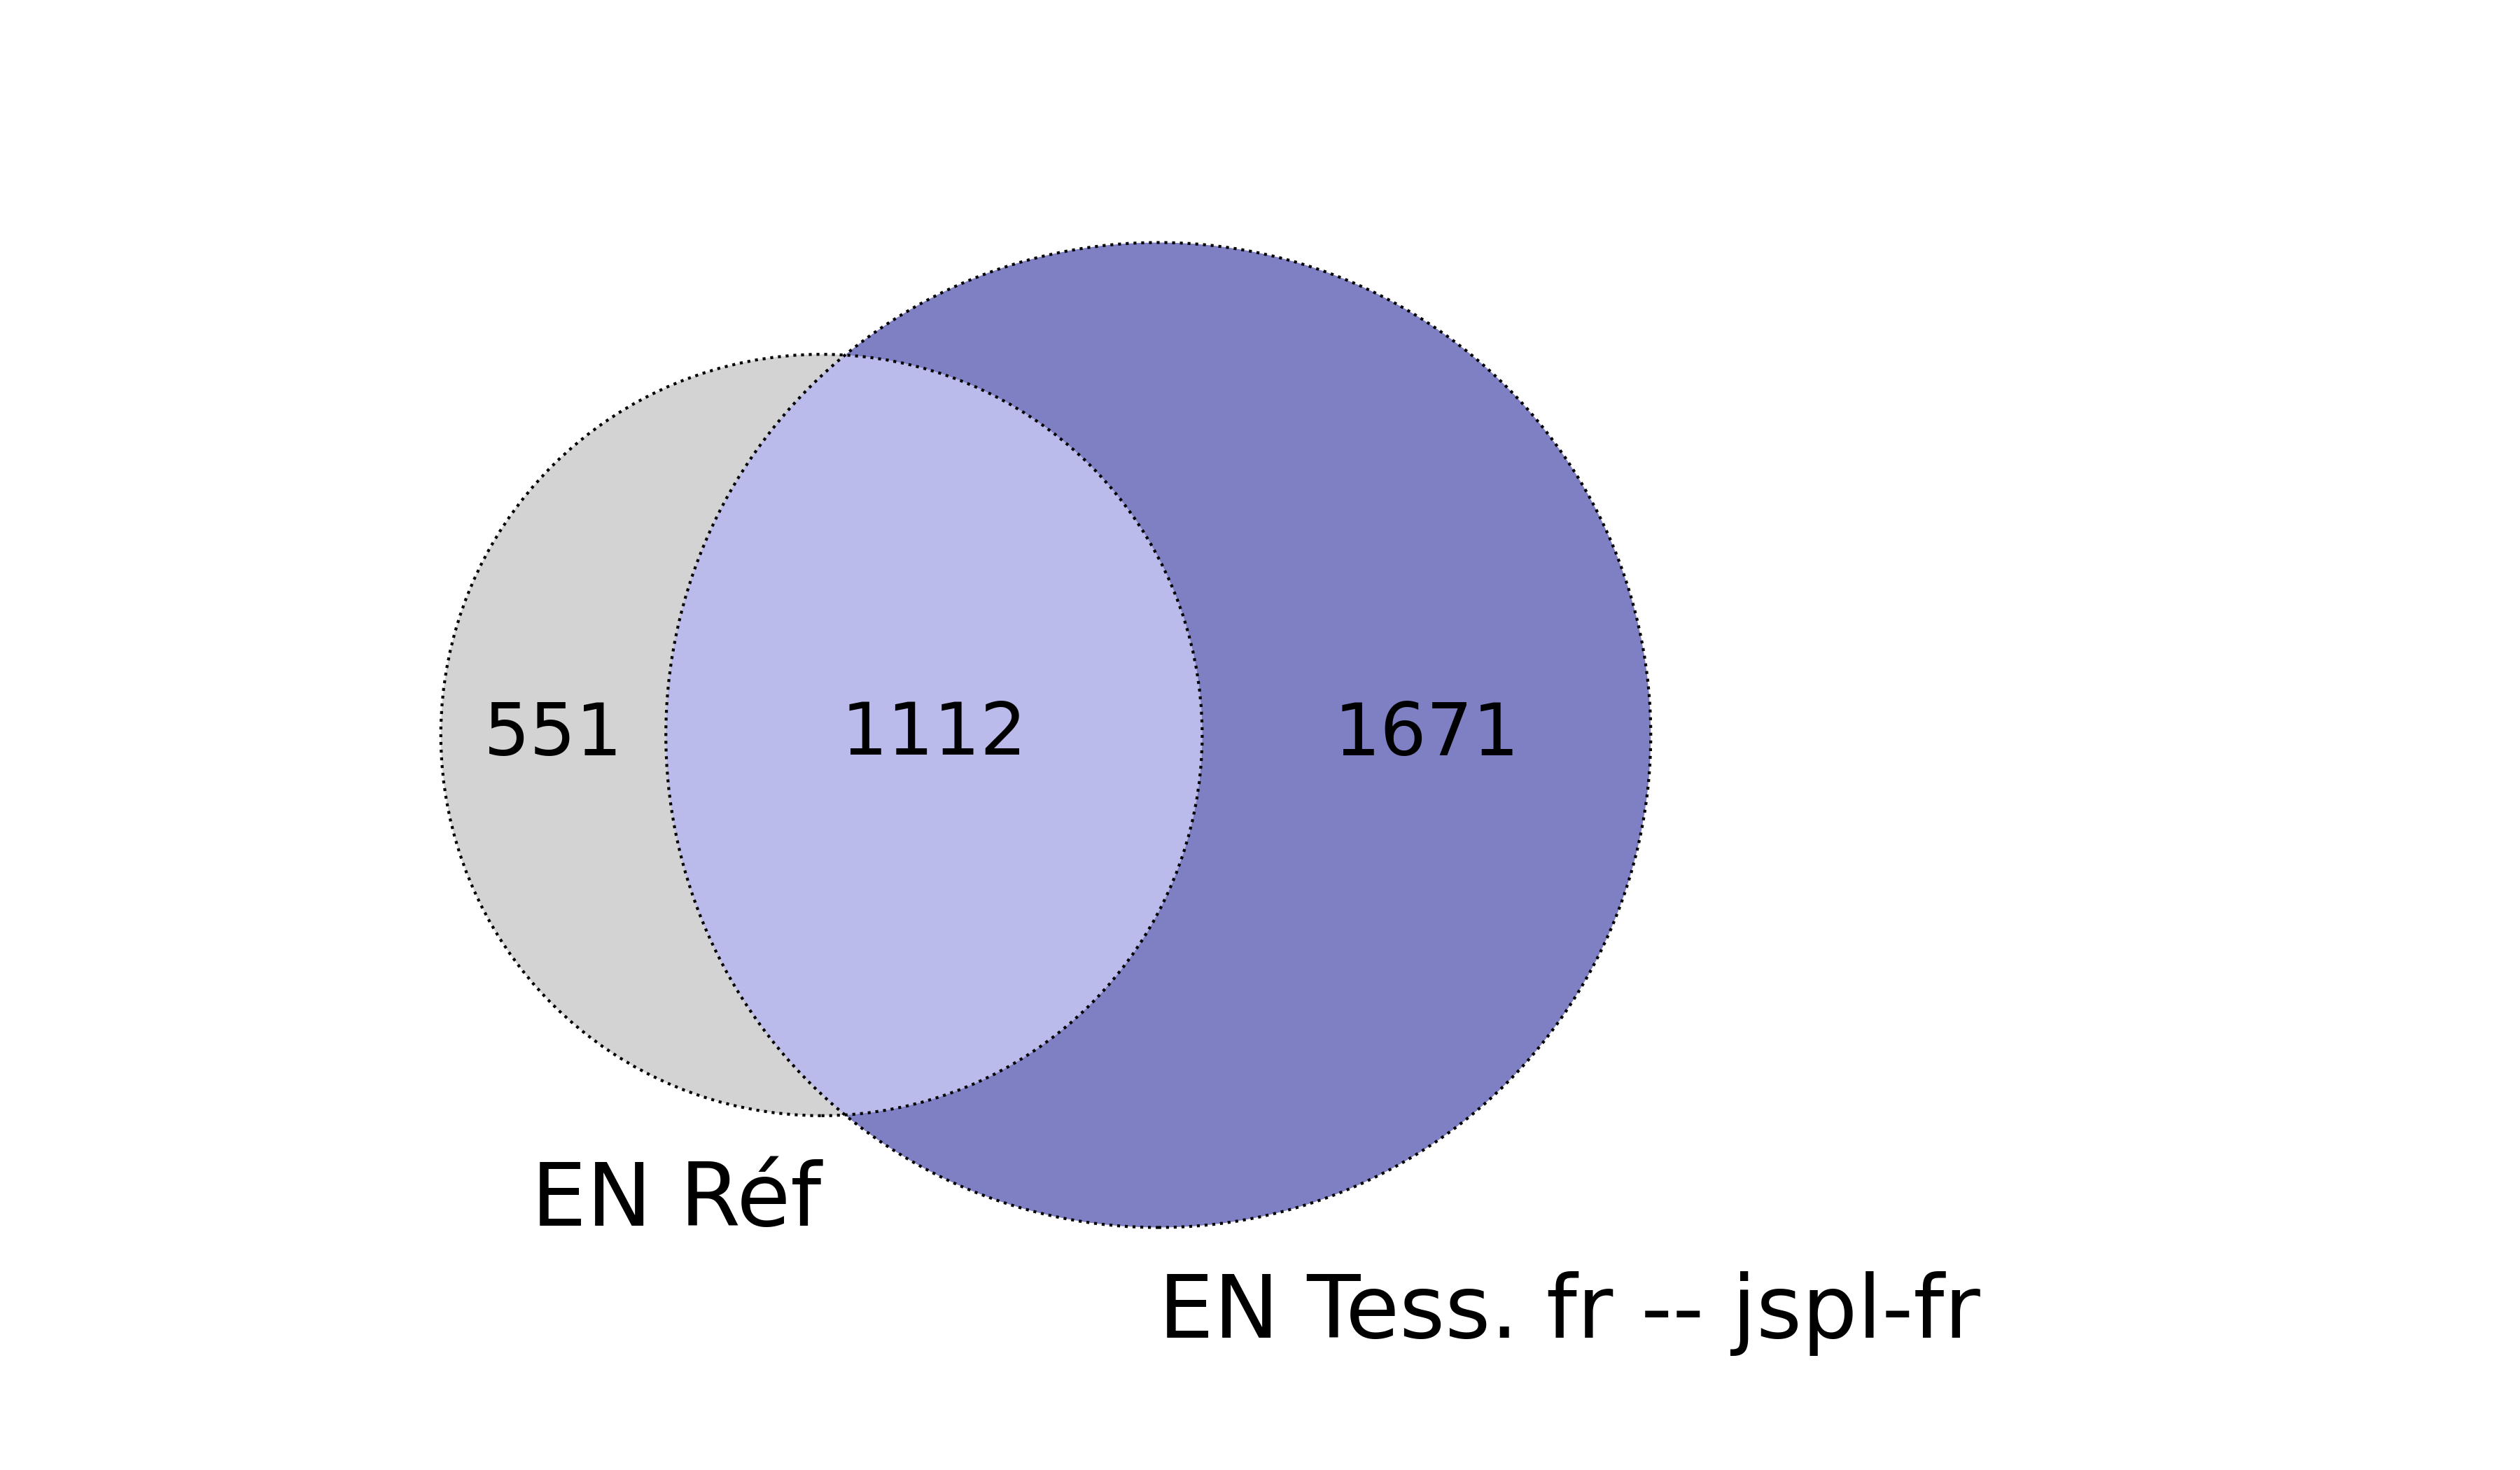
\includegraphics[width=1\textwidth]{IMAGES/INTERSECTIONS_GLOBALES/ELTeCFRA_Tess. fr -- jspl-fr_stanza-concat_intersection.png}
%  \caption{Tess. fr. corrigé -- \texttt{stanza}}
%  \label{fig:ELTeCFRA_Tess. fr -- jspl-fr_stanza-concat_intersection}
%  \end{subfigure}
%    \end{minipage}
%\caption{Intersections pour la configuration Tess-\texttt{spaCy\_lg} corrigées avec le modèle pré-entrainer de JamSpell et le modèle ELTeC, pour le sous-corpus ELTeC français.}
%\label{fig:intersection-globale-tess}
%\end{figure}

Lors du calcul de l'intersection entre les ensembles des EN de référence et des EN issues de ROC, nous rencontrons des problèmes d'alignement. L'alignement strict de l'EN de réf. \textit{Ormeaux} avec l'EN contaminée \textit{Ormaeuux} par la machine n'est pas possible et ce dernier est compté comme FP et ajouté à la liste des hapax, ce qui vient gonfler artificiellement le nombre des FP dans l'ensemble des EN de la ROC. Il s'agit en fait de Faux FP. Enfin, dans l'ensemble des EN reconnues sur les versions de ROC nous remarquons que la majorité des EN présentes dans les résultats obtenus sur la ROC sont effectivement présentes dans les résultats obtenus sur les versions de référence, comme le présente le tableau \ref{tab:FP_VP}. Il n'y a donc pas de véritable déperdition des VP. Enfin, il peut arriver plus rarement que des entités ne soient pas détectées sur la version de Réf. mais le soient sur la version de ROC. Il ne s'agit pas véritablement de FP, mais d'une erreur du système même en contexte non bruité.



En regard des différentes observations que nous venons d'apporter et parce que nous souhaitons rendre compte de la complexité de ces cas réels, nous proposons d'établir une typologie pour l'évaluation des contaminations de ROC sur la REN, élargissant la classification standard des vrais/faux positifs/négatifs. Si les FP sont qualifiés de bruit et les FN de silence, nous avons repéré qu'il existe différents types de bruit et de silence. %Cette typologie permet d'établir quels sont les vrais bruits autrement dit les Vrai FP et les vrais silences (Vrai VN). 


\begin{itemize}


	\item[] \textsc{Cas attendus}
	
	
	\begin{description}

		\item[Vrais positifs (VP)]: EN détectées dans les deux versions.
		\item[Vrais négatifs (VN)]: Aucune EN à reconnaître dans les deux versions.
		\item[Faux positif (FP)]: EN détectées à tort dans la version de ROC (bruit de la REN).
		\item[Faux négatif (FN)]: EN manquantes dans la version de ROC (silence de la REN).
	\end{description}
	
		
	\item[] \textsc{Sous évaluation du bruit et du silence de la REN}
	
	
	\begin{description}
	
		\item[Faux vrais positifs (FVP)]: EN détectées à tort dans les deux versions.
	
	 	\item[Faux vrais négatifs (FVN)] : EN manquantes dans les deux versions.
	 \end{description}
	 
	 \item[] \textsc{sur évaluation du bruit et du silence de la REN}
	
	\begin{description}
	
		\item[Faux faux positifs (FFP)]: EN détectées dans les versions de ROC mais pas dans le texte de référence (EN manquantes dans la référence$^{(i)}$ ou EN contaminées détectées dans la version de ROC$^{(ii)}$).
		
 		\item[Faux faux négatifs (FFN)]: EN  détectées à tort dans le texte de référence.

	\end{description}

\end{itemize}

%\begin{description}
%
%  \item[Vrais vrais positifs VP (VVP)]: EN correctement détectées dans les deux versions.
%  
%  %\item[Vrais vrais négatifs VN (VVN)]: Aucune EN n'est détectée par le système dans aucune version du texte, car il n'y en a pas.
%
%  \item[Vrais faux positifs FP (VFP)]: VRAI BRUIT EN détectées  à tort dans la version de ROC
%
%  \item[Vrais faux négatifs FN (VFN)]:  SILENCE EN détectées dans le texte de référence mais non détecté à tort dans la version de ROC.

%__________________________


%  \item[Faux vrais positifs (FVP)]:  BRUIT EN incorrectement détectées dans les deux versions.

%  \item[Faux vrais négatifs (FVN)] :  Silence total EN manquantes à tort dans les deux versions du texte.
%  

%  
%  \item[Faux faux négatifs (FFN)]: FAUX SILENCE EN  détectées à tort dans le texte de référence mais pas dans les versions de ROC.
%  

%    \item[Faux faux positifs (FFP)]: FAUX BRUIT EN détectées à raison dans les versions de ROC mais non détectées dans le texte de référence (silence dans la référence ou EN contaminées détectées dans la version de ROC).
%
%    
%\end{description}

Il existe un dernier cas des EN qui n'ont pas été transcrites par l'outil de ROC mais qui sont dans la Réf. Cette dernière catégorie est problématique car il ne s'agit pas véritable d'un FN de l'outil de REN, mais d'un FN de l'outil de ROC. 

Le cas de la version Kraken de Reynolds mets en exergue cette observation. Nous avons constaté que seuls 111 types d'EN ont été récupérés dans la configuration Kraken-\texttt{spaCy\_lg}, et pour cause plus de 90\% des pages du PDF n'ont pas été OCRisées très probablement à cause du flou très visible sur les pages concernées. D'autres PDF ont connu le même sort dans de très moindre proportions. De ce fait, une partie des entités manquantes dans les différentes configurations étudiées peuvent être dues non pas à la REN à proprement parler, mais à des transcriptions incomplètes. Nous n'avons pas mesuré l'impact de cette non transcription car il nous est apparu qu'elle était en faible proportion sur tout le corpus et le texte Reynolds était le seul cas très problématique. 


\begin{table}[h!]
    \centering
    %%%%%%%%%% Nouveau tableau sans stanza %%%%%%%%%%%%%%%%

\scriptsize{
\begin{tabular}{|l|l|l|l|}
%p{0.5cm}
\hline
% & \multicolumn{4}{c|}{TGB}\\\cline{2-5}
Type &Version & Contexte & \texttt{spaCy\_lg} \\
\hline
\hline
FVP&Réf. &\textit{[...] better than the milk-and-water lagrime}& lagrime\\
&Kraken &\textit{[...] better than the \textcolor{red}{\_}ilk-
and-water lagrime}& lagrime \\
\hline
FVN&Réf. & \textit{[...] l'été dans leur \textbf{propriété des Peuples}}& \textcolor{red}{()} \\
&Kraken &\textit{[...] l'ete dans leur \textbf{pro-
priete des Peuples}}& \textcolor{red}{()} \\
\hline
\hline
FFP &Réf. &\textit{[...] a sua entrada para o \textbf{colegio militar}}& \textcolor{red}{()} \\
&Kraken &\textit{[...] a s\textcolor{red}{\_}a entrada para
o col\textcolor{red}{c}gio milita}& col\textcolor{red}{c}gio milita \\
FFP &Réf. & \textit{[...] e na vespera delle ir para Coimbra}
&Coimbra \\
&Kraken & \textit{[...] e na vespera delle ir para Coim\textcolor{red}{h}ra} &Coim\textcolor{red}{h}ra \\
\hline
FFN&Réf. & \textit{[...] fleurs emblématiques que les \textcolor{red}{Bachagas}}& \textcolor{red}{Bachagas} \\
&Kraken & \textit{[...] fleurs embl\textcolor{red}{e-}
matiques que les Bach'agas}& () \\
\hline
\end{tabular}}
%\textcolor{red}{} 

%%%%%%%%%% Ancien tableau avec stanza 07/02/2024 %%%%%%%%%%%

%\scriptsize{
%\begin{tabular}{|l|l|l|l|l|}
%%p{0.5cm}
%\hline
%% & \multicolumn{4}{c|}{TGB}\\\cline{2-5}
%Type &Version & Contexte & \texttt{spaCy-lg} &\texttt{stanza}\\
%\hline
%\hline
%FVP&Réf. &\textit{[...] better than the milk-and-water}& lagrime  & ()\\
%&Kraken &\textit{[...] better than the \textcolor{red}{\_}ilk-
%and-water}& lagrime  & () \\
%\hline
%FVN&Réf. & \textit{[...] l'été dans leur \textbf{propriété des Peuples}}& \textcolor{red}{()}  &\textcolor{red}{()} \\
%&Kraken &\textit{[...] l'ete dans leur \textbf{pro-
%priete des Peuples}}& \textcolor{red}{()}  & \textcolor{red}{()}\\
%\hline
%\hline
%FFP $^{(i)}$&Réf. &\textit{[...] a sua entrada para o \textbf{colegio militar}}& \textcolor{red}{()}  & N/A\\
%&Kraken &\textit{[...] a s\textcolor{red}{\_}a entrada para
%o }& col\textcolor{red}{c}gio milita  &N/A \\
%FFP $^{(ii)}$&Réf. & \textit{[...] e na vespera delle ir para}
%&Coimbra& N/A\\
%&Kraken & \textit{[...] e na vespera delle ir para} &Coim\textcolor{red}{h}ra& N/A\\
%\hline
%FFN&Réf. & \textit{[...] fleurs emblématiques que les }& \textcolor{red}{Bachagas} &() \\
%&Kraken & \textit{[...] fleurs embl\textcolor{red}{e-}
%matiques que les Bach'agas}& () &() \\
%\hline
%\end{tabular}}
%%\textcolor{red}{} 

    \caption{Exemples pour la typologie d'évaluation de l'impact des erreurs de ROC sur la REN.}
    \label{tab:typo_eval}
\end{table}

%%%% Matrice mise de côté pour le moment
%En regard des différentes sorties de REN obtenues avec \texttt{spaCy} et \texttt{stanza}, nous proposons une typologie des contaminations de ROC, en élargissant la classification standard des vrais/faux positifs/négatifs. Les définitions correspondant à chaque catégorie (indiquées dans la matrice de confusion, tableau \ref{tab:Matrice_erreur_OCR_V2}) sont les suivantes :
%\begin{table}[H]
 %   \centering
  %  \begin{tabular}{|l|l|l|l|l|}
\hline
EN dans Réf.\ & EN dans la ROC & Éval.$_1$ & Description &  Éval.$_2$ \\
\hline
Oui      & Oui & VP    & Vrai VP & VVP \\ 
\hline
Oui      & Oui & VP    & Bruit dans les deux versions & FVP \\ 
\hline
\hline
%Non        & Non       & VN    & Silence dans les deux versions &  FVN \\
Non        & Non       & VN    & Silence dans les deux versions   & FVN\\ 
\hline
\hline
Oui     & Non         & FN    & Silence dans la ROC & VFN \\ 
\hline
Oui     & Non         & FN    &  Bruit dans la Réf.\ & FFN \\ 
\hline
\hline
Non       & Oui        & FP     &  Bruit dans la ROC & VFP \\
\hline
Non       & Oui        & FP     &  Silence dans la Réf.\ & FFP (VP) \\
\hline
Non       & Oui        & FP     &  Problème de liage d'EN & FFP (VP ?)\\
\hline
\end{tabular}

%%% version anglaise

% \begin{tabular}{|l|l|l|l|l|}
% \hline
% NER in Ref. & NER in OCR & Verdict 1 & Details &  Verdict 2 \\
% \hline
% Yes      & Yes & TP    & True Named Entity & True TP \\ 
% \hline
% Yes      & Yes & TP    & NER Error in Ref. and OCR & False TP  \\ 
% \hline
% \hline
% No        & No       & TN    & No entity in any version   & True TN\\ 
% \hline
% No        & No       & TN    & Missing entity in both versions &  False TN \\ 
% \hline
% \hline
% Yes     & No         & FN    & Missing entity in OCR & True FN \\ 
% \hline
% Yes     & No         & FN    &  Entity error in ref. & False FN \\ 
% \hline
% \hline
% No       & Yes        & FP     &  Entity error in OCR & True FP \\
% \hline
% No       & Yes        & FP     &  Missing entity in Ref. & False FP (TP) \\
% \hline
% No       & Yes        & FP     &  Entity linking issue & False FP (TP ?)\\
% \hline
% \end{tabular}
   % \caption{Typologie des contaminations d'OCR étendue.}
    %\label{tab:my_label}
%\end{table}



%\begin{table}[h!]
%    \centering
%    \scriptsize{\begin{tabular}{|ll|llll|}
\hline
\multicolumn{2}{|l|}{}                                            & \multicolumn{4}{l|}{Réf.}                              \\ 
\cline{3-6} 
\multicolumn{2}{|l|}{\multirow{-2}{*}{}}                    & \multicolumn{1}{l|}{IN}
    & \multicolumn{1}{l|}{\sout{IN}}          
    & \multicolumn{1}{l|}{\sout{OUT}}   
    & \multicolumn{1}{l|}{OUT}      \\ 
\hline
\multicolumn{1}{|l|}{}                      
    & IN                         
    & \multicolumn{1}{l|}{VVP}
    & \multicolumn{1}{l|}{\cellcolor[HTML]{000000}} 
    & FFP   
    %& \multicolumn{1}{l|}{\textcolor{blue}{VFP}}
    & \multicolumn{1}{l|}{\cellcolor[HTML]{000000}}\\ 
\cline{2-6} 
\multicolumn{1}{|l|}{}                      
    & \sout{IN}             
    & \multicolumn{1}{l|}{\cellcolor[HTML]{000000}}  
    & \multicolumn{1}{l|}{FVP}                      
    & \cellcolor[HTML]{000000} 
    & \multicolumn{1}{l|}{VFP}\\ 
\cline{2-6}
\multicolumn{1}{|l|}{\multirow{-4}{*}{ROC}} 
    & \sout{OUT}           
    & \multicolumn{1}{l|}{VFN} 
    & \multicolumn{1}{l|}{\cellcolor[HTML]{000000}} 
    & FVN  
    & \multicolumn{1}{l|}{\cellcolor[HTML]{000000}}                    \\ 
%\hline
\cline{2-6} 
\multicolumn{1}{|l|}{}                      & {\color[HTML]{000000} OUT} 
    %& \multicolumn{1}{l|}{\textcolor{blue}{FN}} 
    & \multicolumn{1}{l|}{\cellcolor[HTML]{000000}}
    & \multicolumn{1}{l|}{FFN} 
    & \cellcolor[HTML]{000000} 
    & \multicolumn{1}{l|}{VVN}\\
\hline
\end{tabular}}

%
%    \caption{Matrice de confusion pour l'évaluation de la REN sur des sorties ROC bruitées. IN = correctement détecté ; \sout{IN} = incorrectement détecté ; OUT = correctement ignoré ; \sout{OUT} = oublié ; case noire = cas impossible}
%    \label{tab:Matrice_erreur_OCR_V2}
%\end{table}

%\begin{table}[]
 %   \centering
  %  \begin{tabular}{|ll|llll|}
\hline
\multicolumn{2}{|l|}{}                                                   & \multicolumn{4}{l|}{Réf.}                                                                                                                                                \\ \cline{3-6} 
\multicolumn{2}{|l|}{\multirow{-2}{*}{}}                                 & \multicolumn{1}{l|}{IN}                       & \multicolumn{1}{l|}{OUT}                      & \multicolumn{1}{l|}{\sout{IN}}          & \sout{OUT}         \\ \hline
\multicolumn{1}{|l|}{}                      & IN                         & \multicolumn{1}{l|}{VP}                       & \multicolumn{1}{l|}{FP}                       & \multicolumn{1}{l|}{\cellcolor[HTML]{000000}} & FFP                      \\ \cline{2-6} 
\multicolumn{1}{|l|}{}                      & {\color[HTML]{000000} OUT} & \multicolumn{1}{l|}{FN}                       & \multicolumn{1}{l|}{VN}                       & \multicolumn{1}{l|}{FFN}                      & \cellcolor[HTML]{000000} \\ \cline{2-6} 
\multicolumn{1}{|l|}{}                      & \sout{IN}             & \multicolumn{1}{l|}{\cellcolor[HTML]{000000}} & \multicolumn{1}{l|}{VFP}                      & \multicolumn{1}{l|}{FVP}                      & \cellcolor[HTML]{000000} \\ \cline{2-6} 
\multicolumn{1}{|l|}{\multirow{-4}{*}{ROC}} & \sout{OUT}           & \multicolumn{1}{l|}{VFP}                      & \multicolumn{1}{l|}{\cellcolor[HTML]{000000}} & \multicolumn{1}{l|}{\cellcolor[HTML]{000000}} & FVN                      \\ \hline
\end{tabular}

   % \caption{Matrice de confusion pour l'évaluation de la REN sur des sorties ROC bruitées. IN = correctement détecté ; \sout{IN} = incorrectement détecté ; OUT = correctement ignoré ; \sout{OUT} = oublié}
    %\label{tab:Matrice_erreur_OCR_V1}
%\end{table}

\subsection{\'Evaluation semi-supervisée des contaminations de ROC sur un corpus annoté}

Afin d'évaluer de manière plus supervisée l'influence du bruit ROC sur la REN nous avons annoté un échantillon du sous-corpus ELTeC français.
 Nous avons choisi de nous limiter aux quatre catégories présentes dans Spacy (Lieux, Personnes, Organisations et Divers).
  Nous avons tout d'abord annoté un échantillon de 3~000 tokens d'une œuvre  puis réalisé une adjudication pour régler les désaccords. 
  Nous avons ensuite annoté 5 000 tokens de 3 versions (Référence, Tesseract et Kraken) de deux œuvres (Daudet et Maupassant)

L'accord inter-annotateur (Kappa de  Fleiss \cite{fleiss2013statistical}) était de $0.877$, significativement plus élevé sur la version de référence ($0.905$) que sur les versions ROC. Nous avons pu observer que les désaccords étaient plus nombreux sur l'annotation des versions océrisées du fait des problèmes de tokenisation.

Grâce à un système de vote majoritaire, nous avons fusionné les annotations pour obtenir un \textit{gold standard} sur chaque version de chaque œuvre.
 Nous avons évalué \texttt{spaCy\_lg} sur cet échantillon, les résultats sont présentés dans le tableau \ref{tab:eval-supervise}.
 En commençant par l'évaluation dite ``GLOBALE'' (tous les types d'entités) nous pouvons remarquer d'une part que les résultats obtenus sur les versions Tesseract sont meilleurs que ceux obtenus sur les versions Kraken. Mais aussi, et ce qui est plus étonnant, que pour ce qui est de l'évaluation souple (où une partie de l'entité suffit à considérer la réponse bonne), que ces résultats sont même meilleurs que ceux obtenus sur la version de référence.
  D'autre part, nous remarquons que là aussi la faiblesse apparente des résultats de REN obtenus sur des versions OCR est principalement due à des problèmes d'alignement entre les tokens contaminés et les tokens de référence. 
\begin{table}[h!]
\scriptsize{\begin{tabular}{l|ccc|ccc}
 %Versions
 &		&	GLOBAL	&		&		&	LIEUX	&		\\
\hline
 \hline
\textbf{Souple}	&	Rappel		&Précision	&	F-Mes.	&	Rappel&		Précision		&F-Mes.	\\
 \hline
Kraken	&	49.57	&	73.72 	&	59.28	&	48.84	&	52.50	&	50.60	\\
													
Tesseract	&	51.53	&	77.63	&	61.94	&	56.41	&	57.89	&	57.14	\\
													
Référence	&	49.78	&	77.55	&	60.64	&	53.49	&	53.49	&	53.49	\\
\hline
\hline
\textbf{Stricte}	&	Rappel		&Précision	&	F-Mes.	&	Rappel&		Précision		&F-Mes.	 \\
\hline
Kraken	&	18.26	&	58.82	&	27.87	&	43.24	&	45.71	&	44.44	\\
Tesseract	&	21.00	&	68.66	&	32.16	&	43.33	&	44.83	&	44.07	\\
Référence	&	21.62	&	69.57	&	32.98	&	41.18	&	45.16	&	43.08	\\
\hline
\hline
\end{tabular}}
\caption{Evaluation de \texttt{spaCy\_lg} sur un échantillon annoté de 10~000 tokens dans trois versions textuelles différentes\label{tab:eval-supervise} en configuration souple et en configuration stricte (GLOBAL: tous les types d'entités), LIEUX: seulement les lieux)}
 \end{table}




